\documentclass[11pt,a4paper,UTF8]{ctexart}

\usepackage[a4paper,margin=2.35cm]{geometry}
\usepackage{amsmath,amssymb,amsthm,mathtools,bm}
\usepackage{graphicx}
\usepackage{booktabs,longtable,array,multirow}
\usepackage{enumitem}
\usepackage{microtype}
\usepackage{setspace}
\usepackage{caption}
\usepackage{subcaption}
\usepackage{float}
\usepackage{xcolor}
\usepackage{hyperref}
\usepackage[numbers,sort&compress]{natbib}
\usepackage{listings}
\usepackage{siunitx}

\graphicspath{{../figures/}}
\setstretch{1.16}
\setlength{\parindent}{2em}
\setlength{\parskip}{0.25em}
\hypersetup{
  colorlinks=true,
  linkcolor=blue!55!black,
  citecolor=blue!55!black,
  urlcolor=blue!55!black,
  pdftitle={不同感染生成与易感耗竭系数下的最优疫情抑制与唯一性},
  pdfauthor={Technical report}
}

\newtheorem{theorem}{定理}[section]
\newtheorem{proposition}[theorem]{命题}
\newtheorem{lemma}[theorem]{引理}
\newtheorem{corollary}[theorem]{推论}
\newtheorem{assumption}[theorem]{假设}
\theoremstyle{definition}
\newtheorem{definition}[theorem]{定义}
\newtheorem{remark}[theorem]{注}

\newcommand{\R}{\mathbb{R}}
\newcommand{\Uad}{\mathcal{U}_{\mathrm{ad}}}
\newcommand{\Fcal}{\mathcal{F}}
\newcommand{\pos}[1]{\left[#1\right]_{+}}
\newcommand{\dd}{\,\mathrm{d}}

\title{\bfseries 不同易感耗竭与感染生成系数下带医疗容量约束的最优疫情抑制\\
\large 结构可解性、全局唯一性、感染成本稳健性与独立控制退化}
\author{技术分析报告}
\date{\today}

\begin{document}
\maketitle

\begin{abstract}
本文研究二维系统
\[
\dot S=-\beta_1(t)SI,\qquad
\dot I=\beta_2(t)SI-\gamma I
\]
在感染容量约束 $I(t)\le K$ 下的最优抑制及唯一性。首先指出：仅仅把原模型中的同一个传播函数拆成两个彼此独立的函数，并继续采用“只惩罚低于自然水平的部分”的线性成本，会产生一个此前模型中不存在的零成本加速通道；在允许 $\beta_1$ 无成本上调时，存在无穷多个零成本可行控制，因此一般意义下的唯一最优控制并不存在。随后提出保持单一社会接触强度的最小结构条件
\[
\beta_1(t)=u(t),\qquad \beta_2(t)=q u(t),\qquad q>0,
\]
其中两条方程中的系数确实不同，但由同一控制驱动。令 $x=qS$ 后，系统严格化为一个守恒结构的受控 SIR 约化系统。本文不依赖原论文的完整 Hamilton--Jacobi 构造，而建立一个新的“校准不变量--成本缺口恒等式”方法：构造
\[
\Fcal(x,I)=I+x-\frac{\gamma}{B}\ln\frac{x}{\gamma/B},
\]
证明任意可行控制的成本与其偏离容量边界的程度、提前抑制、无成本加速以及过度抑制之间存在精确的非负分解。由此直接得到最优策略、最小成本和全局唯一性：先保持自然水平，首次到达 $I=K$ 时发生一次跳跃；随后采用 $u=\gamma/x$ 将感染严格维持在容量上；当 $x=\gamma/B$ 时解除控制。若限制 $0\le u\le B$，该控制在几乎处处意义下全局唯一；若允许 $u>B$ 且不惩罚加速，则唯一性保持到解除时刻，之后与原模型相同存在零成本延拓的非唯一性。本文还给出感染人数成本下策略保持最优的显式阈值、参数比较静态、七组可复现实验，以及独立控制模型的严格退化证明与正则化建模建议。
\end{abstract}

\noindent\textbf{关键词：} 最优控制；状态约束；唯一性；SIR 模型；医疗容量；Hamilton--Jacobi；校准不变量；非唯一性

\tableofcontents
\newpage

\section{问题来源、符号冲突与需要澄清的结构}

附件论文研究了同一个时变接触--感染系数同时出现在易感者减少项和感染者增加项中的系统，并在医疗容量约束和线性抑制成本下解析得到“先不控制--容量边界控制--再解除控制”的策略\citep{MicloSpiroWeibull2022}。本文考虑更一般的形式
\begin{equation}
\begin{cases}
\dot S(t)=-\beta_1(t)S(t)I(t),\\
\dot I(t)=\beta_2(t)S(t)I(t)-\gamma I(t),
\end{cases}
\qquad S(0)=S_0>0,\quad 0<I(0)=I_0<K,
\label{eq:general-model}
\end{equation}
其中 $\gamma>0$ 表示恢复或移除率，$K>0$ 表示医疗容量。为避免与附件中用 $\gamma$ 表示容量的记号冲突，本文始终用 $K$ 表示容量。

式\eqref{eq:general-model}本身还不是一个完整的最优控制问题。至少还需要回答三个问题：
\begin{enumerate}[label=(\roman*),leftmargin=3em]
\item $\beta_1$ 与 $\beta_2$ 是两个独立控制，还是同一个社会接触强度经过两个不同系数映射得到？
\item 自然水平分别是什么，允许不允许超过自然水平，以及超过自然水平是否有成本？
\item 成本是惩罚 $\beta_1$、惩罚 $\beta_2$、惩罚二者之和，还是惩罚其共同的政策强度？
\end{enumerate}
这些选择不是技术细节，而决定唯一性是否可能成立。特别地，当 $\beta_1$ 与 $\beta_2$ 独立，且提高 $\beta_1$ 不付成本时，控制者可以迅速降低 $S$ 而几乎不增加 $I$，从而绕开容量约束；第~\ref{sec:independent-degeneracy}~节将证明此时存在无穷多个零成本最优控制。

本文因此分三层回答问题。
\begin{enumerate}[label=\arabic*.,leftmargin=2.6em]
\item \textbf{精确可解层：} 假设 $\beta_2=q\beta_1$，即两条方程的系数不同但由同一控制驱动。此时给出与附件论文同等级别、但证明方法不同的完整解析理论和唯一性结论。
\item \textbf{任意独立层：} 证明照搬附件的正部成本会导致零成本退化，因而不能期待普适的唯一性定理。
\item \textbf{正则化层：} 给出有界、双向惩罚的独立控制模型、Pontryagin 条件和局部唯一性检验，作为处理真正非比例系数的数值框架。
\end{enumerate}

还应注意，当 $\beta_1\ne\beta_2$ 时
\[
\frac{\dd}{\dd t}(S+I)=(\beta_2-\beta_1)SI-\gamma I,
\]
所以 $S+I$ 不再自动对应一个封闭人群中的“易感+感染”总量。比例参数 $q$ 可解释为感染确认率、潜伏进展率、未观测中间舱室的约化产率，或者两个观测变量量纲不同所产生的转换系数。若 $S$、$I$ 都严格解释为同一总人口的比例，则应在完整模型中加入缺失舱室以恢复质量守恒。

\section{比例但不同的两系数模型：完整最优控制问题}

\subsection{共同控制与成本}

设 $B>0$ 是自然状态下 $\beta_1$ 的水平，$q>0$ 是固定产率比，并令
\begin{equation}
\beta_1(t)=u(t),\qquad \beta_2(t)=q u(t),\qquad
\bar\beta_1=B,\quad \bar\beta_2=qB.
\label{eq:proportional-control}
\end{equation}
允许的控制 $u$ 为局部有界、分段连续函数。主成本取为
\begin{equation}
J(u)=\int_0^\infty \pos{B-u(t)}\dd t,
\label{eq:base-cost}
\end{equation}
并要求状态约束
\begin{equation}
I(t)\le K\qquad \forall t\ge0.
\label{eq:capacity}
\end{equation}
如果政策成本写成两个系数下降量的任意正线性组合，
\[
\int_0^\infty\left[c_1\pos{B-u}+c_2\pos{qB-qu}\right]\dd t
=(c_1+qc_2)J(u),
\]
最优控制完全不变，因此\eqref{eq:base-cost}并不损失一般性。

记 $\Uad(S_0,I_0;K)$ 为满足\eqref{eq:capacity}的可行控制集合，并定义值函数
\begin{equation}
V(S_0,I_0;K)=\inf_{u\in\Uad(S_0,I_0;K)}J(u).
\label{eq:value-def}
\end{equation}
有时还考虑抑制-only 约束
\begin{equation}
0\le u(t)\le B,
\label{eq:suppression-only}
\end{equation}
它排除了无成本“加速传播”。在\eqref{eq:base-cost}下允许 $u>B$ 与附件论文一致；在\eqref{eq:suppression-only}下则能得到解除控制之后的全局唯一性。

\subsection{状态缩放与基础性质}

定义
\begin{equation}
x(t)=qS(t),\qquad x_0=qS_0.
\label{eq:x-transform}
\end{equation}
则\eqref{eq:general-model}--\eqref{eq:proportional-control}严格化为
\begin{equation}
\dot x=-u xI,\qquad \dot I=u xI-\gamma I.
\label{eq:canonical}
\end{equation}
这不是近似，而是精确坐标变换。特别地，两个不同系数模型中的所有控制结论都可以在 $(x,I)$ 平面中证明，再由 $S=x/q$ 还原。

\begin{lemma}[正性、全局存在与耗散]
若 $u\ge0$ 局部有界，则\eqref{eq:canonical}存在唯一全局 Carath\'eodory 解，并且
\begin{equation}
\begin{aligned}
x(t)&=x_0\exp\left(-\int_0^t u(s)I(s)\dd s\right)>0,\\
I(t)&=I_0\exp\left(\int_0^t[u(s)x(s)-\gamma]\dd s\right)>0,\\
\frac{\dd}{\dd t}(x+I)&=-\gamma I\le0.
\end{aligned}
\label{eq:positivity-identities}
\end{equation}
因此 $x(t)+I(t)\le x_0+I_0$，且
\begin{equation}
\int_0^\infty I(t)\dd t\le \frac{x_0+I_0}{\gamma}.
\label{eq:I-integrable-bound}
\end{equation}
\end{lemma}

\begin{proof}
前两个恒等式由分别除以 $x$、$I$ 后积分得到。第三个恒等式由两式相加得到，它同时排除了有限时间爆破。唯一性来自右端关于状态的局部 Lipschitz 性和控制的局部有界性。
\end{proof}

\section{自然传播轨道、峰值与容量是否绑定}

令自然控制为 $u\equiv B$，并定义
\begin{equation}
x_h=\frac{\gamma}{B},\qquad
S_h=\frac{x_h}{q}=\frac{\gamma}{qB}=\frac{\gamma}{\bar\beta_2}.
\label{eq:herd-thresholds}
\end{equation}
在自然传播下，消去时间得到
\begin{equation}
\frac{\dd I}{\dd x}=-1+\frac{x_h}{x},
\end{equation}
从而轨道满足
\begin{equation}
I(x)=I_0+x_0-x+x_h\ln\frac{x}{x_0}.
\label{eq:lf-orbit}
\end{equation}
感染达到峰值时 $\dot I=0$，即 $x=x_h$。若 $x_0\le x_h$，则感染从初始时刻起不增长；若 $x_0>x_h$，自然传播峰值为
\begin{equation}
I_{\mathrm{pk}}
=I_0+x_0-x_h+x_h\ln\frac{x_h}{x_0}.
\label{eq:peak}
\end{equation}
因此：
\begin{equation}
I_{\mathrm{pk}}\le K
\quad\Longrightarrow\quad
u^*(t)\equiv B,\quad V=0.
\label{eq:inactive-case}
\end{equation}
下文集中于容量真正绑定的情形
\begin{equation}
x_0>x_h,\qquad I_{\mathrm{pk}}>K>I_0.
\label{eq:active-assumption}
\end{equation}

自然轨道与 $I=K$ 有两个交点。记较大的横坐标为 $x_1>x_h$，即
\begin{equation}
K=I_0+x_0-x_1+x_h\ln\frac{x_1}{x_0}.
\label{eq:x1-root}
\end{equation}
它对应第一次到达容量的时刻 $\tau_1$。该时刻可由一维积分精确表示为
\begin{equation}
\tau_1=
\int_{x_1}^{x_0}
\frac{\dd x}{B x\left(I_0+x_0-x+x_h\ln(x/x_0)\right)}.
\label{eq:tau1-integral}
\end{equation}
一般没有必要把\eqref{eq:tau1-integral}强行写成特殊函数；数值计算中使用事件定位即可获得高精度结果。

\section{候选最优策略及其闭式表达}

在 $I=K$ 上保持感染不变需要
\[
0=\dot I=(ux-\gamma)K,
\]
因此唯一的切向控制为
\begin{equation}
u=\frac{\gamma}{x}=\frac{\gamma}{qS}.
\label{eq:boundary-control}
\end{equation}
此时
\begin{equation}
\dot x=-\gamma K,
\qquad
x(t)=x_1-\gamma K(t-\tau_1).
\label{eq:linear-boundary-x}
\end{equation}
当 $x$ 降至 $x_h$ 时，$u=\gamma/x_h=B$，容量边界控制与自然控制连续衔接。定义
\begin{equation}
\tau_2=\tau_1+\frac{x_1-x_h}{\gamma K}.
\label{eq:tau2}
\end{equation}

\begin{definition}[容量填充控制]
定义
\begin{equation}
 u^*(t)=
\begin{cases}
B, & 0\le t\le\tau_1,\\[2mm]
\displaystyle\frac{\gamma}{x(t)}
=\frac{B}{1+BK(\tau_2-t)}, & \tau_1<t\le\tau_2,\\[3mm]
B, & t>\tau_2.
\end{cases}
\label{eq:optimal-u}
\end{equation}
相应的两个不同系数为
\begin{equation}
\beta_1^*(t)=u^*(t),\qquad
\beta_2^*(t)=q u^*(t).
\label{eq:optimal-betas}
\end{equation}
\end{definition}

控制在 $\tau_1$ 处从 $B$ 向下跳到 $\gamma/x_1$，随后单调上升，并在 $\tau_2$ 恢复到 $B$。在原变量中，边界段满足
\begin{equation}
I(t)=K,\qquad
S(t)=S_1-\frac{\gamma K}{q}(t-\tau_1),
\qquad S_1=\frac{x_1}{q}.
\label{eq:S-boundary}
\end{equation}

\begin{proposition}[候选策略的可行性与成本]
在\eqref{eq:active-assumption}下，\eqref{eq:optimal-u}满足容量约束，且其成本为
\begin{align}
J(u^*)
&=B(\tau_2-\tau_1)-\frac1K\ln\frac{x_1}{x_h}
\label{eq:cost-x1}\\
&=\frac1K\left[
\frac{B}{\gamma}(I_0+x_0-K)
-\ln\frac{Bx_0}{\gamma}-1
\right].
\label{eq:cost-closed}
\end{align}
\end{proposition}

\begin{proof}
第一阶段自然轨道第一次在 $x=x_1$ 时到达 $I=K$；第二阶段由\eqref{eq:boundary-control}保证 $\dot I=0$；第三阶段从 $(x_h,K)$ 出发，在自然控制下有 $\dot I\le0$。边界段上利用 $\dd t=-\dd x/(\gamma K)$ 得
\[
J(u^*)=\int_{x_h}^{x_1}\frac{B-\gamma/x}{\gamma K}\dd x,
\]
即\eqref{eq:cost-x1}。再用\eqref{eq:x1-root}消去 $x_1$ 即得\eqref{eq:cost-closed}。
\end{proof}

\section{新的校准不变量方法：最优性与唯一性的直接证明}
\label{sec:calibration}

附件论文采用 Hamilton--Jacobi 验证。下面给出一个更短且能量化唯一性的不同方法。

\subsection{校准函数}
定义
\begin{equation}
\Fcal(x,I)=I+x-x_h\ln\frac{x}{x_h},
\qquad x_h=\frac{\gamma}{B}.
\label{eq:calibration-F}
\end{equation}
自然控制 $u=B$ 时 $\dot\Fcal=0$。临界自然轨道在 $(x_h,K)$ 处与容量线相切，因此其校准水平为
\begin{equation}
\Fcal_c=K+x_h.
\label{eq:Fcritical}
\end{equation}
初始值为
\begin{equation}
\Fcal_0=I_0+x_0-x_h\ln\frac{x_0}{x_h}.
\label{eq:F0}
\end{equation}
容量绑定条件等价于 $\Fcal_0>\Fcal_c$。

对任意控制，记
\begin{equation}
L(t)=\pos{B-u(t)},\qquad A(t)=\pos{u(t)-B}.
\label{eq:L-A}
\end{equation}
于是 $B-u=L-A$，直接计算得到关键恒等式
\begin{equation}
\boxed{
\dot\Fcal(t)=-x_h L(t)I(t)+x_h A(t)I(t).
}
\label{eq:F-derivative}
\end{equation}
它说明：抑制使校准水平下降，无成本加速使其上升；每单位抑制成本所产生的有效校准下降与当时感染水平 $I$ 成正比。因此，在 $I\le K$ 的限制下，最有效的抑制只能发生在 $I=K$。

\subsection{有限成本轨道必然到达临界横坐标}

\begin{lemma}[临界横坐标到达引理]
设 $u$ 可行且 $J(u)<\infty$。则 $x(t)$ 的极限满足
\begin{equation}
x_\infty:=\lim_{t\to\infty}x(t)\le x_h.
\label{eq:xinf-le-xh}
\end{equation}
令 $\sigma$ 表示第一次到达 $x\le x_h$ 的时刻；若仅渐近到达，则把 $\sigma=\infty$ 并按极限解释。总有
\begin{equation}
\Fcal(x(\sigma),I(\sigma))\le\Fcal_c.
\label{eq:F-sigma}
\end{equation}
\end{lemma}

\begin{proof}
$x$ 单调不增，故极限存在。若 $x_\infty>x_h$，则存在 $T$、$c>0$ 使 $Bx(t)-\gamma\ge c$ 对 $t\ge T$ 成立。由 $u=B-L+A\ge B-L$，
\[
\ln\frac{I(t)}{I(T)}
=\int_T^t[u(s)x(s)-\gamma]\dd s
\ge c(t-T)-x_0\int_T^tL(s)\dd s.
\]
因 $\int_0^\infty L=J(u)<\infty$，右端趋于 $+\infty$，与 $I(t)\le K$ 矛盾，故\eqref{eq:xinf-le-xh}成立。若在有限时刻穿过 $x_h$，则当时 $I\le K$，从而
$\Fcal\le K+x_h$；若渐近到达，则取极限得到同一结论。
\end{proof}

\subsection{成本缺口恒等式}

\begin{theorem}[最优成本及定量缺口]
在\eqref{eq:active-assumption}下，对任意有限成本可行控制 $u$，有
\begin{equation}
J(u)\ge J^*:=\frac{\Fcal_0-\Fcal_c}{x_hK},
\label{eq:lower-bound-J}
\end{equation}
且 $J^*$ 与\eqref{eq:cost-closed}完全相同。更精确地，取上一引理中的 $\sigma$，则
\begin{align}
J(u)-J^*
={}&\int_0^\sigma L(t)\left(1-\frac{I(t)}K\right)\dd t
+\int_\sigma^\infty L(t)\dd t
\notag\\
&+\frac{\Fcal_c-\Fcal(x(\sigma),I(\sigma))}{x_hK}
+\frac1K\int_0^\sigma A(t)I(t)\dd t.
\label{eq:gap-identity}
\end{align}
右端每一项都非负。
\end{theorem}

\begin{proof}
积分\eqref{eq:F-derivative}至 $\sigma$ 得
\begin{equation}
\int_0^\sigma L I\dd t
=\frac{\Fcal_0-\Fcal(\sigma)}{x_h}
+\int_0^\sigma A I\dd t.
\label{eq:LI-identity}
\end{equation}
另一方面，
\[
J(u)=\int_0^\sigma L\left(1-\frac IK\right)\dd t
+\frac1K\int_0^\sigma LI\dd t
+\int_\sigma^\infty L\dd t.
\]
代入\eqref{eq:LI-identity}并减去
$J^*=(\Fcal_0-\Fcal_c)/(x_hK)$，即得\eqref{eq:gap-identity}。由 $I\le K$ 和\eqref{eq:F-sigma}可知各项非负。
\end{proof}

式\eqref{eq:gap-identity}不仅证明最优性，而且把次优性的来源完全分开：
\begin{itemize}[leftmargin=2.2em]
\item 第一项是\textbf{提前或低于容量时抑制}的浪费；
\item 第二项是越过临界横坐标之后仍继续抑制的浪费；
\item 第三项是把系统推到临界自然轨道以下的\textbf{过度抑制}；
\item 第四项是容量解除前无成本加速造成的额外负担。
\end{itemize}

\begin{corollary}[全局唯一性]
在\eqref{eq:active-assumption}下：
\begin{enumerate}[label=(\roman*),leftmargin=3em]
\item 在允许 $u\ge0$ 且成本为\eqref{eq:base-cost}时，任意最优控制都与\eqref{eq:optimal-u}在 $[0,\tau_2]$ 上几乎处处相同；在 $t>\tau_2$，任意满足可行性的零成本延拓 $u(t)\ge B$ 都保持最优。
\item 若加入抑制-only 约束\eqref{eq:suppression-only}，则 $u^*$ 在 $[0,\infty)$ 上几乎处处唯一。
\item 若对 $u>B$ 加入任意严格正的附加成本，则唯一的最优后续同样是 $u=B$，从而恢复全局唯一性。
\end{enumerate}
\label{cor:uniqueness}
\end{corollary}

\begin{proof}
最优时\eqref{eq:gap-identity}右端必须全部为零。于是容量解除前不能有 $A>0$；$L>0$ 只能发生在 $I=K$；到达 $x_h$ 时必须恰有 $I=K$；之后不能再有 $L>0$。在首次到达容量之前 $I<K$，故 $L=A=0$，从而 $u=B$。在 $I=K$ 且 $x>x_h$ 上，可行性要求 $u\le\gamma/x<B$；为了不离开容量边界而产生第一项的严格正损失，只能取切向值 $u=\gamma/x$。这一直持续到 $x=x_h$。若 $u\le B$，解除后零成本条件强制 $u=B$；若允许 $u>B$ 且不收费，则只要后续仍可行即可产生多重延拓。
\end{proof}

\begin{corollary}[唯一性的定量稳定性]
设某个可行策略在集合 $E\subset[0,\sigma]$ 上满足 $I(t)\le K-\eta$，且在 $E$ 上有抑制量 $L(t)>0$，其中 $\eta>0$。则
\begin{equation}
J(u)-J^*\ge\frac{\eta}{K}\int_E L(t)\dd t.
\label{eq:early-suppression-gap}
\end{equation}
因此“稍微提前一点抑制”并非同成本替代，而有可计算的一阶成本缺口。
\end{corollary}

\section{Hamilton--Jacobi 交叉验证}

校准证明已经给出全局结论。为与附件论文的框架对应，下面给出简洁的 HJB 验证。对 $x>x_h$ 且自然轨道将超过容量的区域，候选值函数为
\begin{equation}
V(x,I)=\frac{\Fcal(x,I)-\Fcal_c}{x_hK}
=\frac1K\left[
\frac{B}{\gamma}(I+x-K)-\ln\frac{Bx}{\gamma}-1
\right].
\label{eq:value-explicit}
\end{equation}
在自然传播安全集上取 $V=0$。在活动区域
\begin{equation}
V_x=\frac{1-x_h/x}{x_hK},\qquad
V_I=\frac1{x_hK}.
\label{eq:value-gradient}
\end{equation}
Hamiltonian 为
\begin{equation}
H(x,I,p)=\inf_{u\ge0}
\left[-p_xuxI+p_I(uxI-\gamma I)+\pos{B-u}\right].
\label{eq:Hamiltonian}
\end{equation}
代入\eqref{eq:value-gradient}后，在 $0\le u\le B$ 上 Hamiltonian 可写为
\[
(B-u)\left(1-\frac{I}{K}\right),
\]
而在 $u\ge B$ 上可写为 $(u-B)I/K$。因此当 $I<K$ 时唯一极小点是 $u=B$。在容量边界 $I=K$ 上，点态 HJB 极小集合与可行集合相交为 $[0,\gamma/x]$；HJB 本身并不选择其中唯一一点，必须再结合动态规划等号轨道或成本缺口恒等式，才得到唯一切向值 $u=\gamma/x$。这个计算与\eqref{eq:gap-identity}一致，但后者进一步给出了全局成本缺口和唯一性来源。

\section{加入感染人数成本后的稳健性}

考虑
\begin{equation}
J_a(u)=J(u)+a\int_0^\infty I(t)\dd t,
\qquad a\ge0.
\label{eq:infection-cost}
\end{equation}
由于坐标变换\eqref{eq:x-transform}把模型精确化为附件模型，感染成本的阈值理论可以完整移植。令 $\lambda\in(0,x_h)$ 是方程
\begin{equation}
\lambda=x_h\left[\ln\frac{\lambda}{x_h}+1\right]+K
\label{eq:lambda-equation}
\end{equation}
的较小根。它是从 $(x_h,K)$ 出发，之后采用自然控制时的最终 $x$ 水平。令 $\rho\in(0,1)$ 是
\begin{equation}
\rho^2+\rho+\ln(1-\rho)=0
\label{eq:rho-equation}
\end{equation}
的唯一非零根，数值上 $\rho\approx0.6838026238$，并定义
\begin{equation}
K_0=\rho^2x_h.
\label{eq:K0}
\end{equation}

\begin{theorem}[感染成本稳健阈值]
容量填充控制\eqref{eq:optimal-u}在成本\eqref{eq:infection-cost}下保持最优，当且仅当
\begin{equation}
0\le a\le a_0(K),
\label{eq:a-range}
\end{equation}
其中
\begin{equation}
 a_0(K)=
\begin{cases}
\displaystyle\frac{\gamma-B\lambda}{K\lambda}, & K\le K_0,\\[3mm]
\displaystyle\frac{B\rho}{(1-\rho)K_0}, & K>K_0.
\end{cases}
\label{eq:a0}
\end{equation}
在该范围内，最优值为
\begin{equation}
J_a^*=J^*+\frac{a}{\gamma}(x_0+I_0-\lambda).
\label{eq:Ja-star}
\end{equation}
\end{theorem}

\begin{proof}
定义自然传播安全集 $\mathcal A$ 为从给定状态出发采用 $u\equiv B$ 后永不触及 $I=K$ 的状态集合。对 $(x,I)\in\mathcal A$，令 $\ell(x,I)\in(0,x_h)$ 表示自然传播下的最终 $x$ 水平。由自然轨道不变量，$\ell$ 是方程
\begin{equation}
\ell-x_h\ln\ell=I+x-x_h\ln x
\label{eq:ell-implicit}
\end{equation}
的较小根。容量填充策略对应的候选值函数为
\begin{equation}
V_a(x,I)=
\begin{cases}
\displaystyle V(x,I)+\frac a\gamma(x+I-\lambda), &(x,I)\notin\mathcal A,\\[2mm]
\displaystyle \frac a\gamma(x+I-\ell(x,I)), &(x,I)\in\mathcal A,
\end{cases}
\label{eq:Va-candidate}
\end{equation}
其中 $V$ 是\eqref{eq:value-explicit}。在活动区，附加项对两个状态分量的梯度增量相同，且
$\dot x+\dot I=-\gamma I$，故它与运行成本中的 $aI$ 精确抵消；因此原来的 Hamilton--Jacobi 等式继续成立。

下面检查安全集。对\eqref{eq:ell-implicit}隐式求导，得到
\begin{equation}
\ell_x=\frac{1-x_h/x}{1-x_h/\ell},
\qquad
\ell_I=\frac{1}{1-x_h/\ell}.
\label{eq:ell-gradient}
\end{equation}
将 $p=\nabla V_a$ 代入含感染成本的 Hamiltonian，可化为
\begin{equation}
H_a(x,I,\nabla V_a)
=B\left[\min\{1,Z(x,I)\}-Z(x,I)\right],
\qquad
Z(x,I)=\frac{aI\ell(x,I)}{\gamma-B\ell(x,I)}.
\label{eq:Ha-safe}
\end{equation}
所以 HJB 等式在整个安全集成立的充要条件是
\begin{equation}
a\,M(K)\le1,
\qquad
M(K):=\sup_{(x,I)\in\mathcal A}
\frac{I\ell(x,I)}{\gamma-B\ell(x,I)}.
\label{eq:M-condition}
\end{equation}

为计算 $M(K)$，固定最终水平 $\ell\in(0,x_h)$。当 $\ell\le\lambda$ 时，同一最终水平曲线在安全集中的最大感染值为 $K$，且
$K\ell/(\gamma-B\ell)$ 随 $\ell$ 增加，因此该部分的最大值在 $\ell=\lambda$ 取得。对 $\ell>\lambda$，最大感染值在 $x=x_h$ 处取得，并等于
\begin{equation}
\chi(\ell)=\ell-x_h-x_h\ln\frac{\ell}{x_h}.
\label{eq:chi-ell}
\end{equation}
令 $r=1-\ell/x_h\in(0,1)$，则
\begin{equation}
\frac{\chi(\ell)\ell}{\gamma-B\ell}
=\frac{\gamma}{B^2}f(r),
\qquad
f(r)=(r-1)\left(1+\frac{\ln(1-r)}r\right),
\label{eq:F-r-infection}
\end{equation}
且
\begin{equation}
f'(r)=\frac{r^2+r+\ln(1-r)}{r^2}.
\label{eq:fprime-infection}
\end{equation}
由 $\rho^2+\rho+\ln(1-\rho)=0$，$f$ 在 $(0,\rho)$ 上严格增加、在 $(\rho,1)$ 上严格下降。再注意
$K=x_h[-r_\lambda-\ln(1-r_\lambda)]$，故 $K\le K_0$ 等价于 $r_\lambda\le\rho$。于是
\begin{equation}
M(K)=
\begin{cases}
\displaystyle\frac{K\lambda}{\gamma-B\lambda}, & K\le K_0,\\[3mm]
\displaystyle\frac{(1-\rho)K_0}{B\rho}, & K>K_0.
\end{cases}
\label{eq:M-explicit}
\end{equation}
由\eqref{eq:M-condition}可知临界值必须是 $a_0=1/M(K)$，即\eqref{eq:a0}。若 $a>a_0$，则安全集中存在状态使\eqref{eq:Ha-safe}严格为负，沿相应 Hamiltonian 改进方向可降低成本，故容量填充策略不再最优；这也给出必要性。

最后，由\eqref{eq:positivity-identities}，
\[
\int_0^\infty I(t)\dd t
=\frac{x_0+I_0-x_\infty}{\gamma}.
\]
容量填充策略的最终状态为 $(\lambda,0)$，从而得到\eqref{eq:Ja-star}。
\end{proof}

\begin{remark}
对 $0\le a<a_0$，活动区内的 Hamiltonian 极小点保持严格，故推论~\ref{cor:uniqueness} 关于首次到达容量和容量边界段的唯一性仍成立。临界值 $a=a_0$ 处可能出现额外的并列极小状态；若要求严格全局唯一，宜取 $a<a_0$ 并采用 $0\le u\le B$ 或对加速施加正成本。
\end{remark}

\begin{proposition}[感染成本阈值关于容量的单调性]
在 $0<K<K_0$ 上，$a_0(K)$ 严格递减；在 $K\ge K_0$ 上，$a_0(K)$ 为常数。因此医疗容量越紧，容量填充策略对附加感染成本的稳健区间越宽。
\end{proposition}

\begin{proof}
令
\begin{equation}
r=1-\frac{B\lambda}{\gamma}\in(0,\rho].
\label{eq:r-lambda}
\end{equation}
由\eqref{eq:lambda-equation}可得
\begin{equation}
K=\frac{\gamma}{B}\left[-r-\ln(1-r)\right],
\qquad
\frac{\dd K}{\dd r}=\frac{\gamma}{B}\frac{r}{1-r}>0.
\label{eq:K-r}
\end{equation}
在第一分支上，结合\eqref{eq:F-r-infection}可写成
\begin{equation}
a_0(K)=\frac{B^2}{\gamma}\frac1{f(r)}.
\label{eq:a0-r-correct}
\end{equation}
由\eqref{eq:fprime-infection}知 $f'(r)>0$ 于 $(0,\rho)$，故 $a_0$ 随 $r$ 严格下降；再由\eqref{eq:K-r}即得 $\dd a_0/\dd K<0$。在 $K=K_0$ 时两分支连续相接，之后由\eqref{eq:a0}第二分支可知其为常数。
\end{proof}

\begin{remark}[对附件公式的内部一致性核查]
附件正文显示的阈值式（其式(25)）把 $a_0$ 写成了\eqref{eq:M-explicit}右端本身；但其附录 HJB 计算要求
$aI\ell/(\gamma-B\ell)\le1$，并进一步计算了该比值的上确界。因此阈值应为该上确界的倒数，即\eqref{eq:a0}。这一修正同时与量纲、附件随后声称的“容量增加时阈值递减”以及直接数值验证一致。本文图形和程序采用经 HJB 推导核验后的倒数公式。
\end{remark}

\section{比较静态与生物学解释}

所有比例差异通过
\begin{equation}
x_0=qS_0,
\label{eq:q-x0}
\end{equation}
进入解析公式。以下导数均在容量绑定区域内理解。

\subsection{系数比 \texorpdfstring{$q$}{q}}
由\eqref{eq:peak}，
\begin{equation}
\frac{\partial I_{\mathrm{pk}}}{\partial q}
=S_0-\frac{x_h}{q}
=S_0-\frac{\gamma}{Bq}>0
\label{eq:peak-q-derivative}
\end{equation}
只要 $qS_0>x_h$。最小成本对 $q$ 的导数为
\begin{equation}
\frac{\partial J^*}{\partial q}
=\frac1K\left(\frac{BS_0}{\gamma}-\frac1q\right)
=\frac{1}{Kq}\left(\frac{BqS_0}{\gamma}-1\right)>0.
\label{eq:cost-q-derivative}
\end{equation}
因此，感染生成相对于易感耗竭越强，峰值越高，达到容量越早，且最低控制成本越大。

\subsection{容量 \texorpdfstring{$K$}{K}}
写
\begin{equation}
A(q)=\frac{B}{\gamma}(I_0+qS_0)-\ln\frac{BqS_0}{\gamma}-1,
\end{equation}
则 $J^*=A(q)/K-B/\gamma$，故
\begin{equation}
\frac{\partial J^*}{\partial K}=-\frac{A(q)}{K^2}<0,
\qquad
\frac{\partial^2 J^*}{\partial K^2}=\frac{2A(q)}{K^3}>0.
\label{eq:capacity-comparative}
\end{equation}
容量扩张降低最小抑制成本，但边际收益递减。

\subsection{初始感染与解除阈值}
有
\begin{equation}
\frac{\partial J^*}{\partial I_0}=\frac{B}{\gamma K}>0.
\label{eq:I0-comparative}
\end{equation}
而解除阈值
\[
S_h=\frac{\gamma}{\bar\beta_2}
\]
只依赖恢复率和感染生成系数的自然水平，不依赖 $\beta_1$ 的绝对尺度。这意味着在比例模型中，决定感染能否在无控制下下降的是 $\bar\beta_2S<\gamma$；$\beta_1$ 影响的是沿容量边界消耗易感者的速度和控制持续时间。

\section{两个完全独立控制时的零成本退化}
\label{sec:independent-degeneracy}

现在真正把 $\beta_1$、$\beta_2$ 视为独立控制。设自然水平为 $B_1,B_2>0$，并照搬附件论文的“只惩罚下降”思想：
\begin{equation}
J_{\mathrm{ind}}(\beta_1,\beta_2)
=\int_0^\infty
\left[w_1\pos{B_1-\beta_1(t)}+w_2\pos{B_2-\beta_2(t)}\right]\dd t,
\qquad w_1,w_2>0.
\label{eq:independent-cost}
\end{equation}

\begin{theorem}[独立控制的零成本非唯一性]
假设
\begin{equation}
S_0>\frac{\gamma}{B_2},\qquad 0<I_0<K.
\label{eq:degenerate-assumption}
\end{equation}
若允许 $\beta_1>B_1$ 且超过自然水平不收费，则存在无穷多个彼此不同的可行控制，使
\begin{equation}
J_{\mathrm{ind}}=0.
\label{eq:zero-cost}
\end{equation}
即使自然控制 $(B_1,B_2)$ 会突破容量，最优值仍为零，且最优控制不唯一。
\end{theorem}

\begin{proof}
任取目标 $S_T\in(0,\gamma/B_2)$。选取足够小的 $\delta>0$，使
\begin{equation}
I_0\exp\left(\pos{B_2S_0-\gamma}\delta\right)<K.
\label{eq:delta-small}
\end{equation}
在 $[0,\delta]$ 上令
\begin{equation}
\beta_2(t)=B_2,
\qquad \beta_1(t)=M>B_1.
\label{eq:acceleration-pulse}
\end{equation}
由 $S(t)\le S_0$，
\[
I(t)\le I_0e^{(B_2S_0-\gamma)t}<K.
\]
另一方面 $\dot I\ge-\gamma I$，故 $I(t)\ge I_0e^{-\gamma t}$，从而
\[
S(\delta)
=S_0\exp\left(-M\int_0^\delta I(t)\dd t\right)
\le S_0\exp\left[-M\frac{I_0(1-e^{-\gamma\delta})}{\gamma}\right].
\]
取
\begin{equation}
M\ge
\max\left\{B_1,
\frac{\gamma\ln(S_0/S_T)}{I_0(1-e^{-\gamma\delta})}
\right\}
\label{eq:M-choice}
\end{equation}
即可保证 $S(\delta)\le S_T$。在 $t>\delta$ 令 $(\beta_1,\beta_2)=(B_1,B_2)$，则
\[
\dot I\le(B_2S_T-\gamma)I<0,
\]
所以容量永不再被威胁。全过程中 $\beta_1\ge B_1$、$\beta_2=B_2$，故\eqref{eq:independent-cost}为零。改变 $\delta$ 和 $M$ 即得到无穷多个不同的零成本可行控制。
\end{proof}

该结论解释了为什么原论文中“允许无成本加速”并未破坏前两阶段唯一性，而在\eqref{eq:general-model}中却会彻底破坏唯一性：原模型提高同一个 $b$ 时，易感者消耗和新感染同时加速；这里提高 $\beta_1$ 只减少 $S$，却不直接增加 $I$，形成了一个不符合质量守恒的免费通道。

\subsection{恢复可解释性和唯一性的三种办法}

\begin{enumerate}[label=\arabic*.,leftmargin=2.6em]
\item \textbf{共同控制耦合：} 采用本文主模型 $\beta_2=q\beta_1$。这是保留闭式解和全局唯一性的最小条件。
\item \textbf{对双向偏离都收费并设置上界：} 例如 $0\le\beta_i\le M_i$，成本使用 $(\beta_i-B_i)^2$，从而消除无成本加速。
\item \textbf{补全舱室：} 若 $\beta_1\ne\beta_2$ 源于未观测的暴露者、隔离者或报告率，应引入相应状态，使易感者流失的去向明确，而不是把两条流量独立指定。
\end{enumerate}

\section{真正非比例情形的正则化最优控制框架}

当 $\beta_1$、$\beta_2$ 必须独立估计时，可以在有限决策窗口 $[0,T]$ 上采用
\begin{equation}
\begin{aligned}
J_{\mathrm{reg}}(\beta_1,\beta_2)
={}&\int_0^T\left[
\frac{c_1}{2}(\beta_1-B_1)^2
+\frac{c_2}{2}(\beta_2-B_2)^2
+\omega I(t)
\right]\dd t,\\
&0\le\beta_i(t)\le M_i,
\qquad I(t)\le K.
\end{aligned}
\label{eq:regularized-problem}
\end{equation}
由于控制集合紧、右端对状态连续且线性依赖控制，标准 Filippov--Cesari 理论保证最优控制存在\citep{Cesari1983,Liberzon2012}。

在非活动容量区间，Hamiltonian 为
\begin{equation}
\begin{aligned}
\mathcal H={}&
\frac{c_1}{2}(\beta_1-B_1)^2
+\frac{c_2}{2}(\beta_2-B_2)^2+\omega I\\
&-\lambda_S\beta_1SI
+\lambda_I(\beta_2SI-\gamma I).
\end{aligned}
\label{eq:regularized-H}
\end{equation}
相应伴随方程为
\begin{equation}
\begin{cases}
\dot\lambda_S=\beta_1I\lambda_S-\beta_2I\lambda_I,\\
\dot\lambda_I=-\omega+\beta_1S\lambda_S-(\beta_2S-\gamma)\lambda_I,
\end{cases}
\label{eq:adjoint}
\end{equation}
而点态唯一的 Hamiltonian 极小控制为
\begin{equation}
\begin{aligned}
\beta_1^*(t)&=\Pi_{[0,M_1]}
\left(B_1+\frac{\lambda_SSI}{c_1}\right),\\
\beta_2^*(t)&=\Pi_{[0,M_2]}
\left(B_2-\frac{\lambda_ISI}{c_2}\right).
\end{aligned}
\label{eq:projection-controls}
\end{equation}
若 $I=K$ 上存在边界弧，则可行性要求
\begin{equation}
\beta_2\le\frac{\gamma}{S},
\label{eq:independent-boundary-viability}
\end{equation}
保持在边界上时取等号；状态约束乘子会在进入和离开边界时引起 $\lambda_I$ 的跳跃条件。

严格凸的瞬时成本保证给定状态--伴随变量时控制唯一，但由于状态方程非线性，它本身并不自动保证整个最优轨道全局唯一。实际计算中应检查二阶充分条件：若约化目标在临界锥上满足
\begin{equation}
\delta^2J_{\mathrm{reg}}[h,h]\ge c\|h\|_{L^2(0,T)}^2,
\qquad c>0,
\label{eq:second-order-condition}
\end{equation}
则所得极值解是严格局部唯一的。较大的 $c_1,c_2$、较短的 $T$ 和不太强的非线性通常有利于\eqref{eq:second-order-condition}成立。与比例模型不同，一般非比例模型没有只依赖四个基本参数的统一闭式策略。

\section{数值方法、参数与结果}

\subsection{算法}

比例模型的数值计算不需要离散优化：
\begin{enumerate}[label=\arabic*.,leftmargin=2.6em]
\item 用\eqref{eq:peak}判断容量是否绑定；
\item 用一维求根得到 $x_1$ 或 $S_1$；
\item 用带事件的 ODE 积分得到 $\tau_1$；
\item 用\eqref{eq:tau2}、\eqref{eq:optimal-u}显式构造边界段；
\item 用\eqref{eq:cost-closed}和直接积分双重校验成本。
\end{enumerate}
所有图均提供相互独立的 Python 与 MATLAB 程序。

\subsection{基准参数}

\begin{table}[H]
\centering
\caption{比例两系数模型的基准参数与主要输出。}
\label{tab:baseline-parameters}
\begin{tabular}{lll}
\toprule
量 & 数值 & 含义\\
\midrule
$B$ & $1.0$ & $\beta_1$ 的自然水平\\
$q$ & $0.8$ & $\beta_2/\beta_1$\\
$\bar\beta_2$ & $0.8$ & 感染生成系数自然水平\\
$\gamma$ & $0.3$ & 恢复率\\
$(S_0,I_0)$ & $(0.99,0.01)$ & 初始状态\\
$K$ & $0.15$ & 医疗容量\\
$S_h$ & $0.375000$ & 解除控制阈值\\
$I_{\rm pk}$ & $0.210766$ & 无控制峰值\\
$S_1$ & $0.666787$ & 首次到达容量时的易感比例\\
$\tau_1$ & $6.659464$ & 容量进入时刻\\
$\tau_2$ & $11.846795$ & 解除控制时刻\\
$J^*$ & $1.350363$ & 最小抑制成本\\
$S_\infty^*$ & $0.113141$ & 最优策略下最终易感比例\\
\bottomrule
\end{tabular}
\end{table}

直接数值积分
\(
\int_{\tau_1}^{\tau_2}(B-u^*)\dd t
\)
得到 $1.350362774500724$，与闭式公式\eqref{eq:cost-closed}的差小于 $10^{-12}$。

\subsection{相平面与时间轨道}

\begin{figure}[H]
\centering
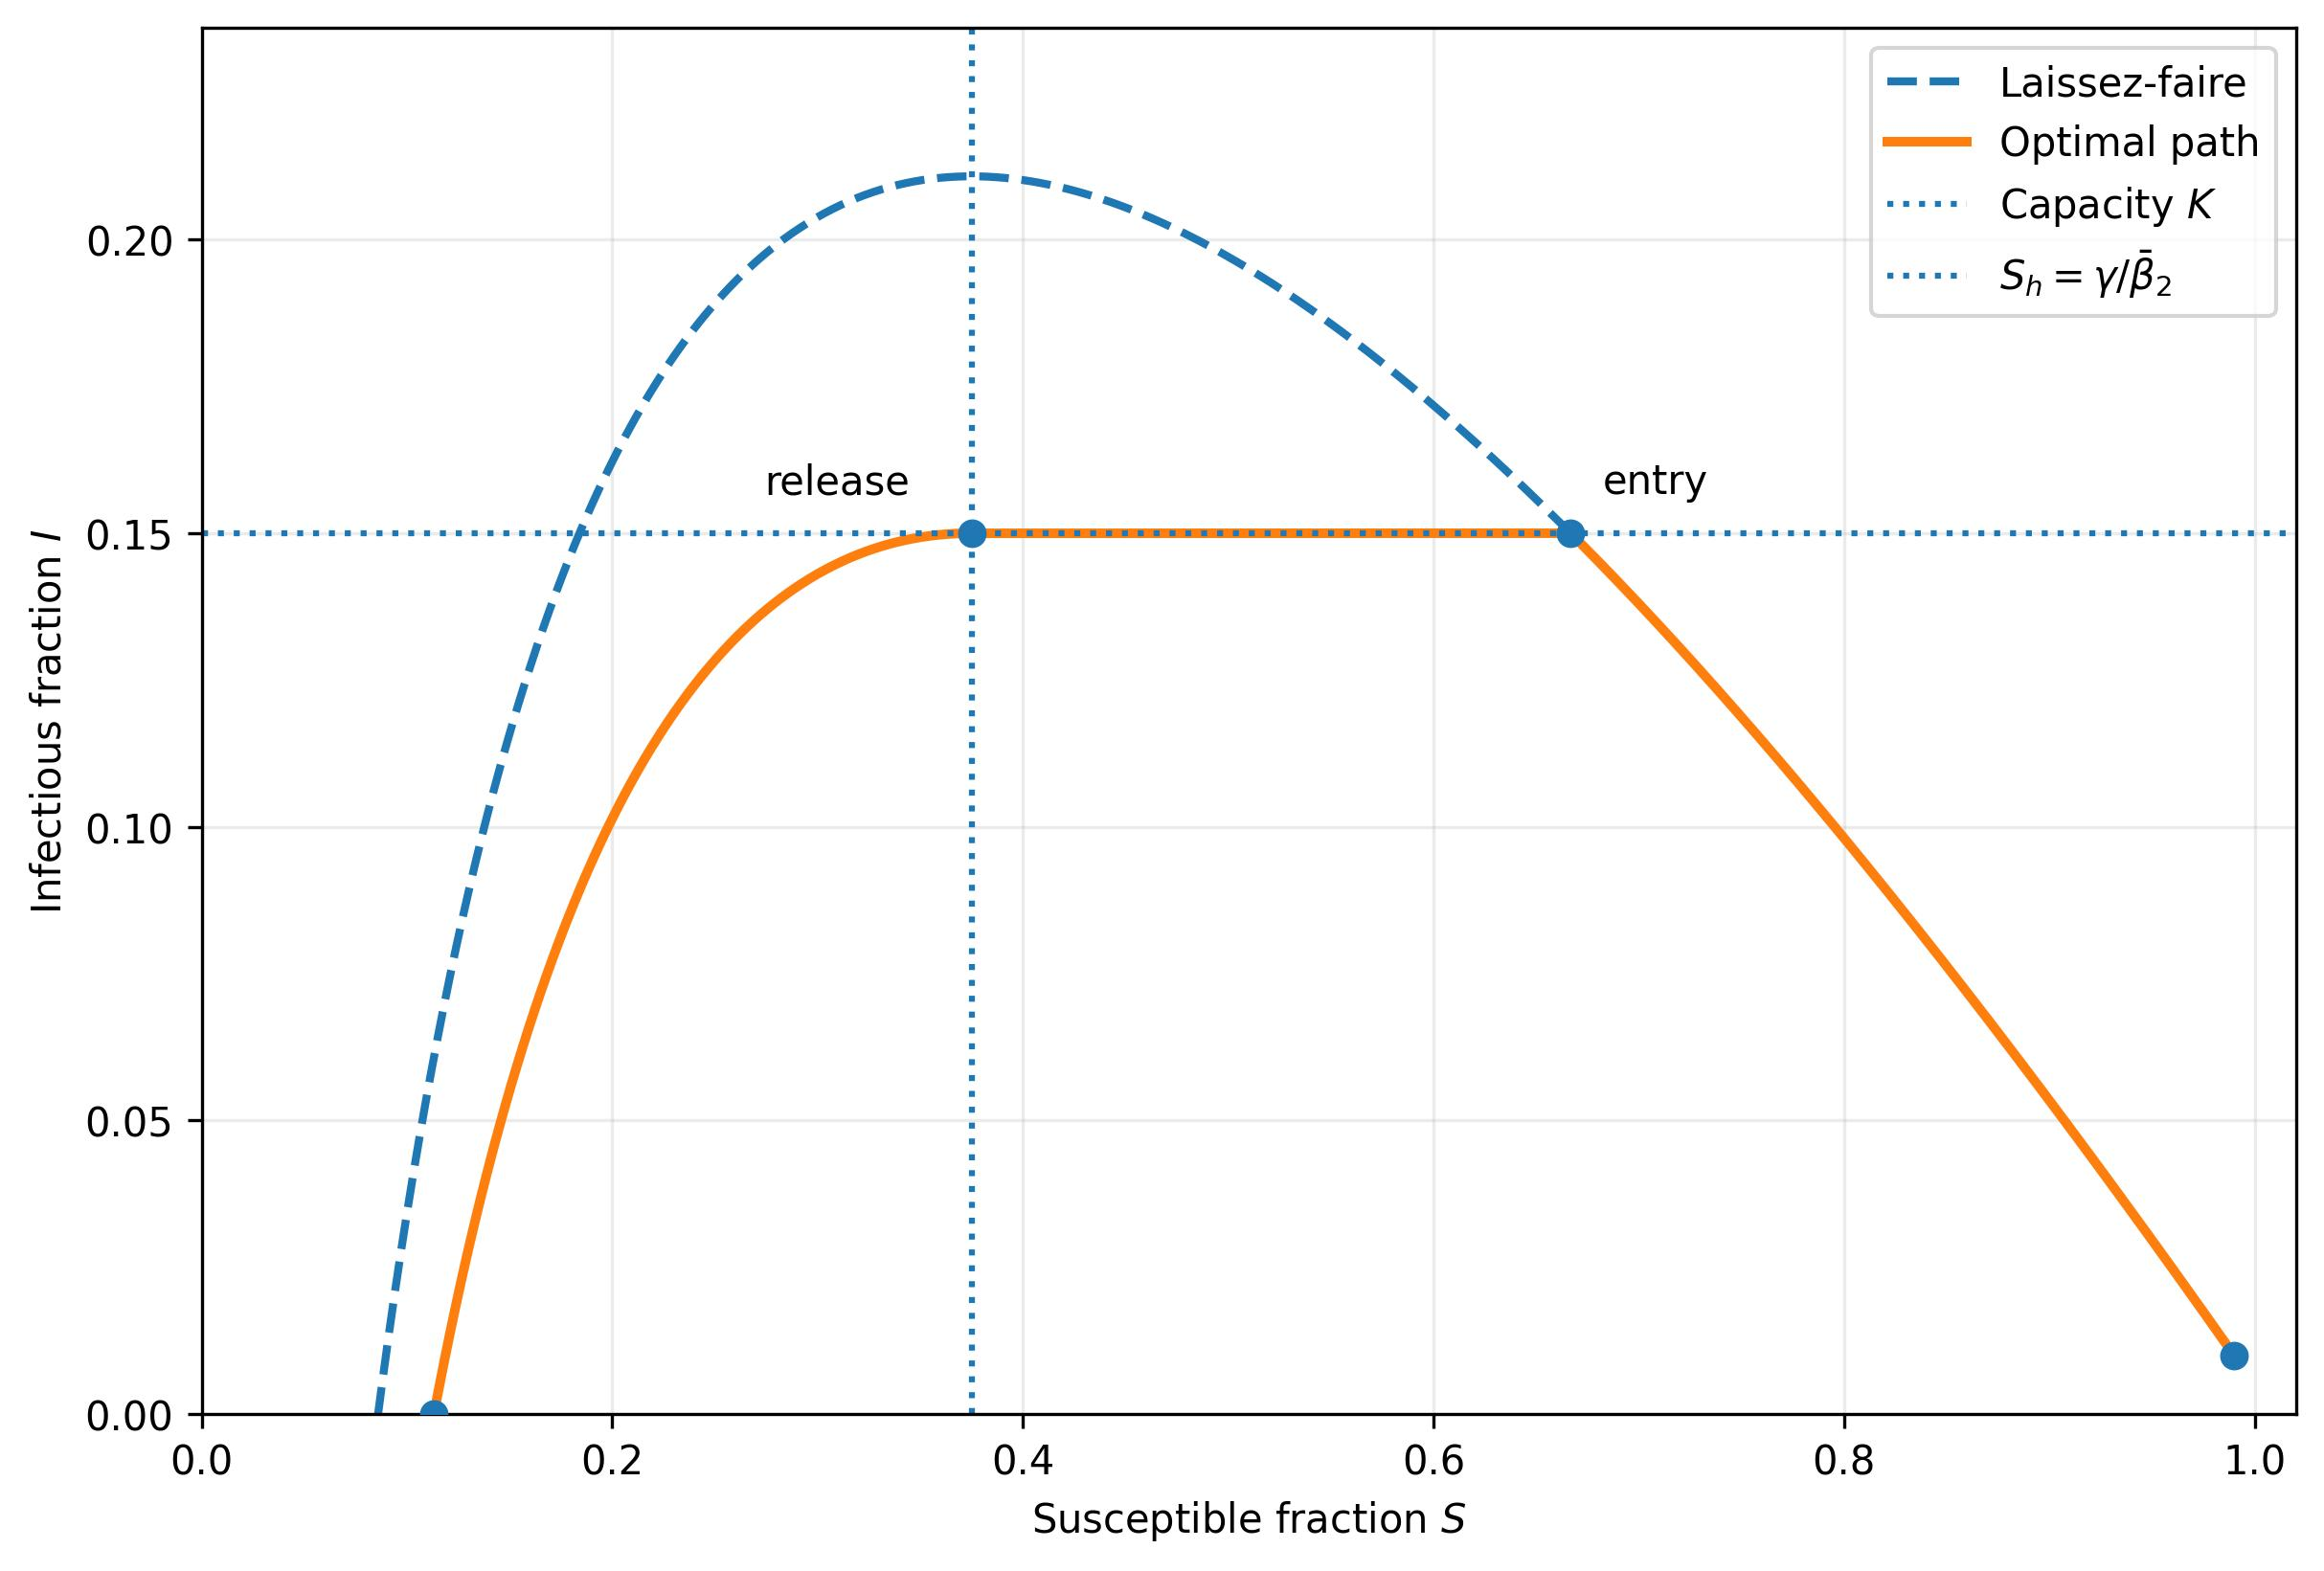
\includegraphics[width=0.92\textwidth]{Figure_1_phase_plane.jpg}
\caption{比例但不同系数模型的相平面。虚线为自然传播轨道；实线为最优轨道。最优轨道首先沿自然轨道到达 $I=K$，随后沿容量线向左移动，至 $S=S_h$ 后回到自然轨道。}
\label{fig:phase-plane}
\end{figure}

\begin{figure}[H]
\centering
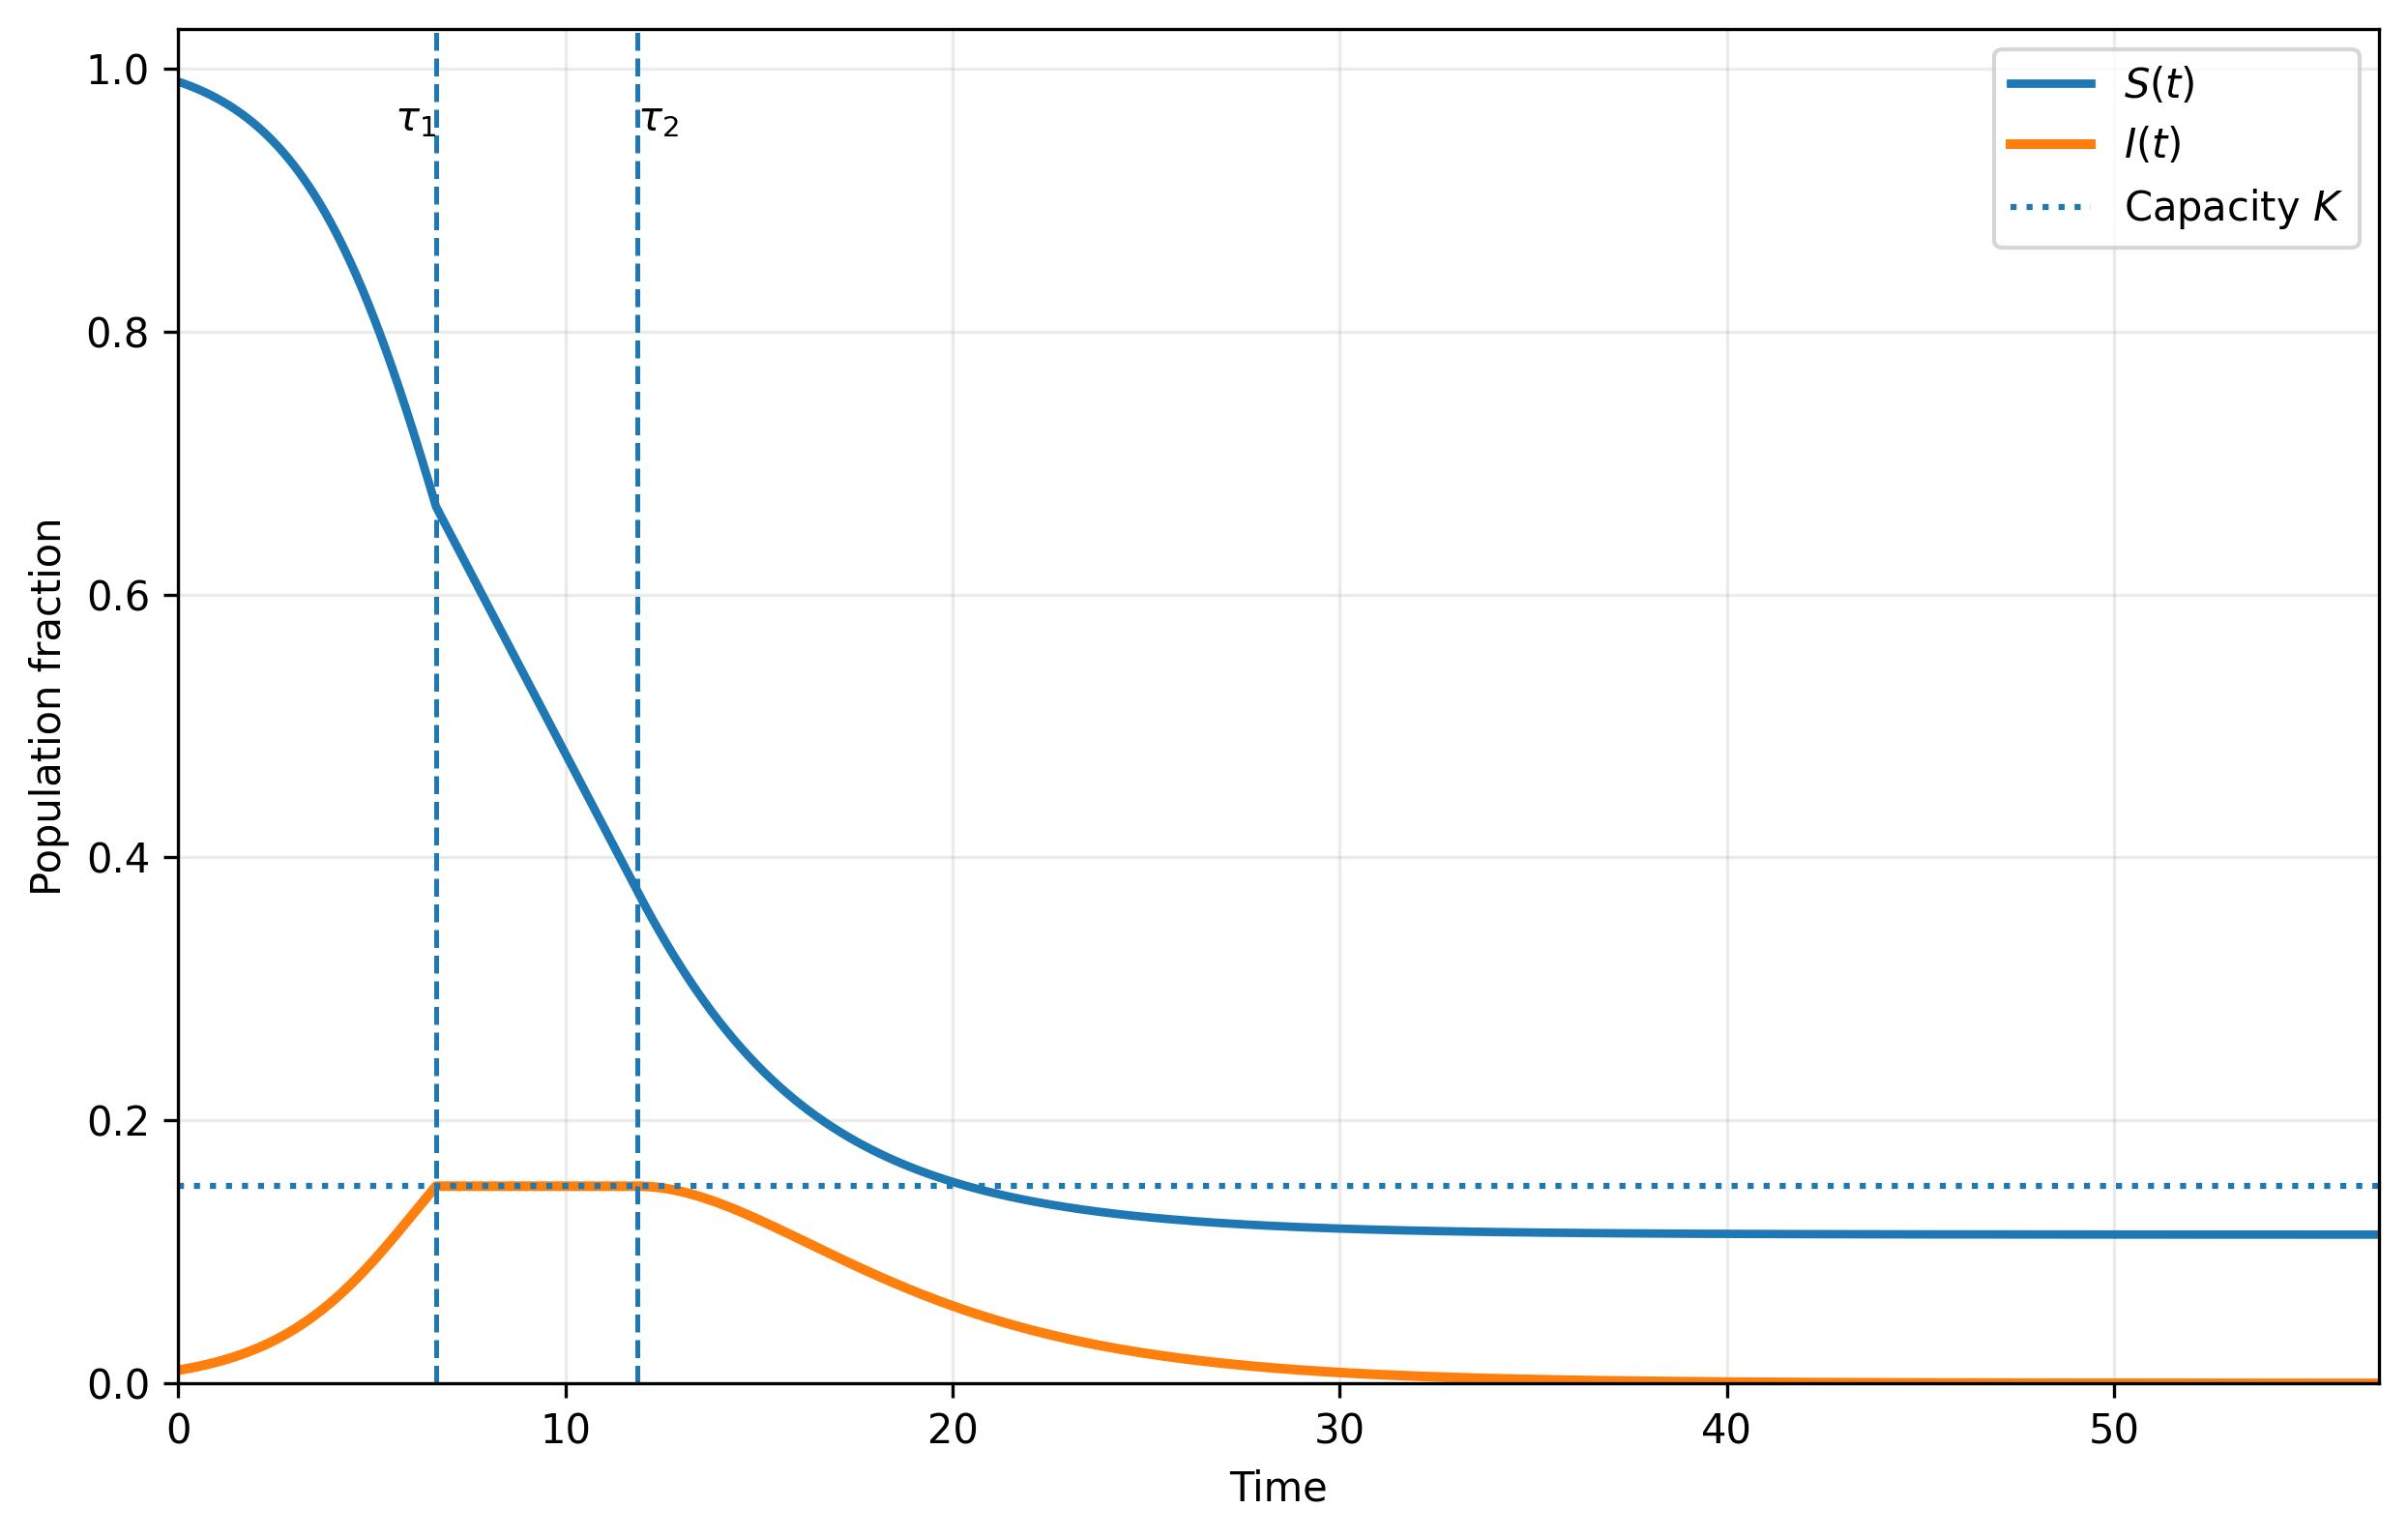
\includegraphics[width=0.92\textwidth]{Figure_2_state_time_series.jpg}
\caption{最优策略下 $S(t)$ 与 $I(t)$。感染在 $[\tau_1,\tau_2]$ 上严格等于容量 $K$；$S$ 在该阶段线性下降。}
\label{fig:state-time}
\end{figure}

\begin{figure}[H]
\centering
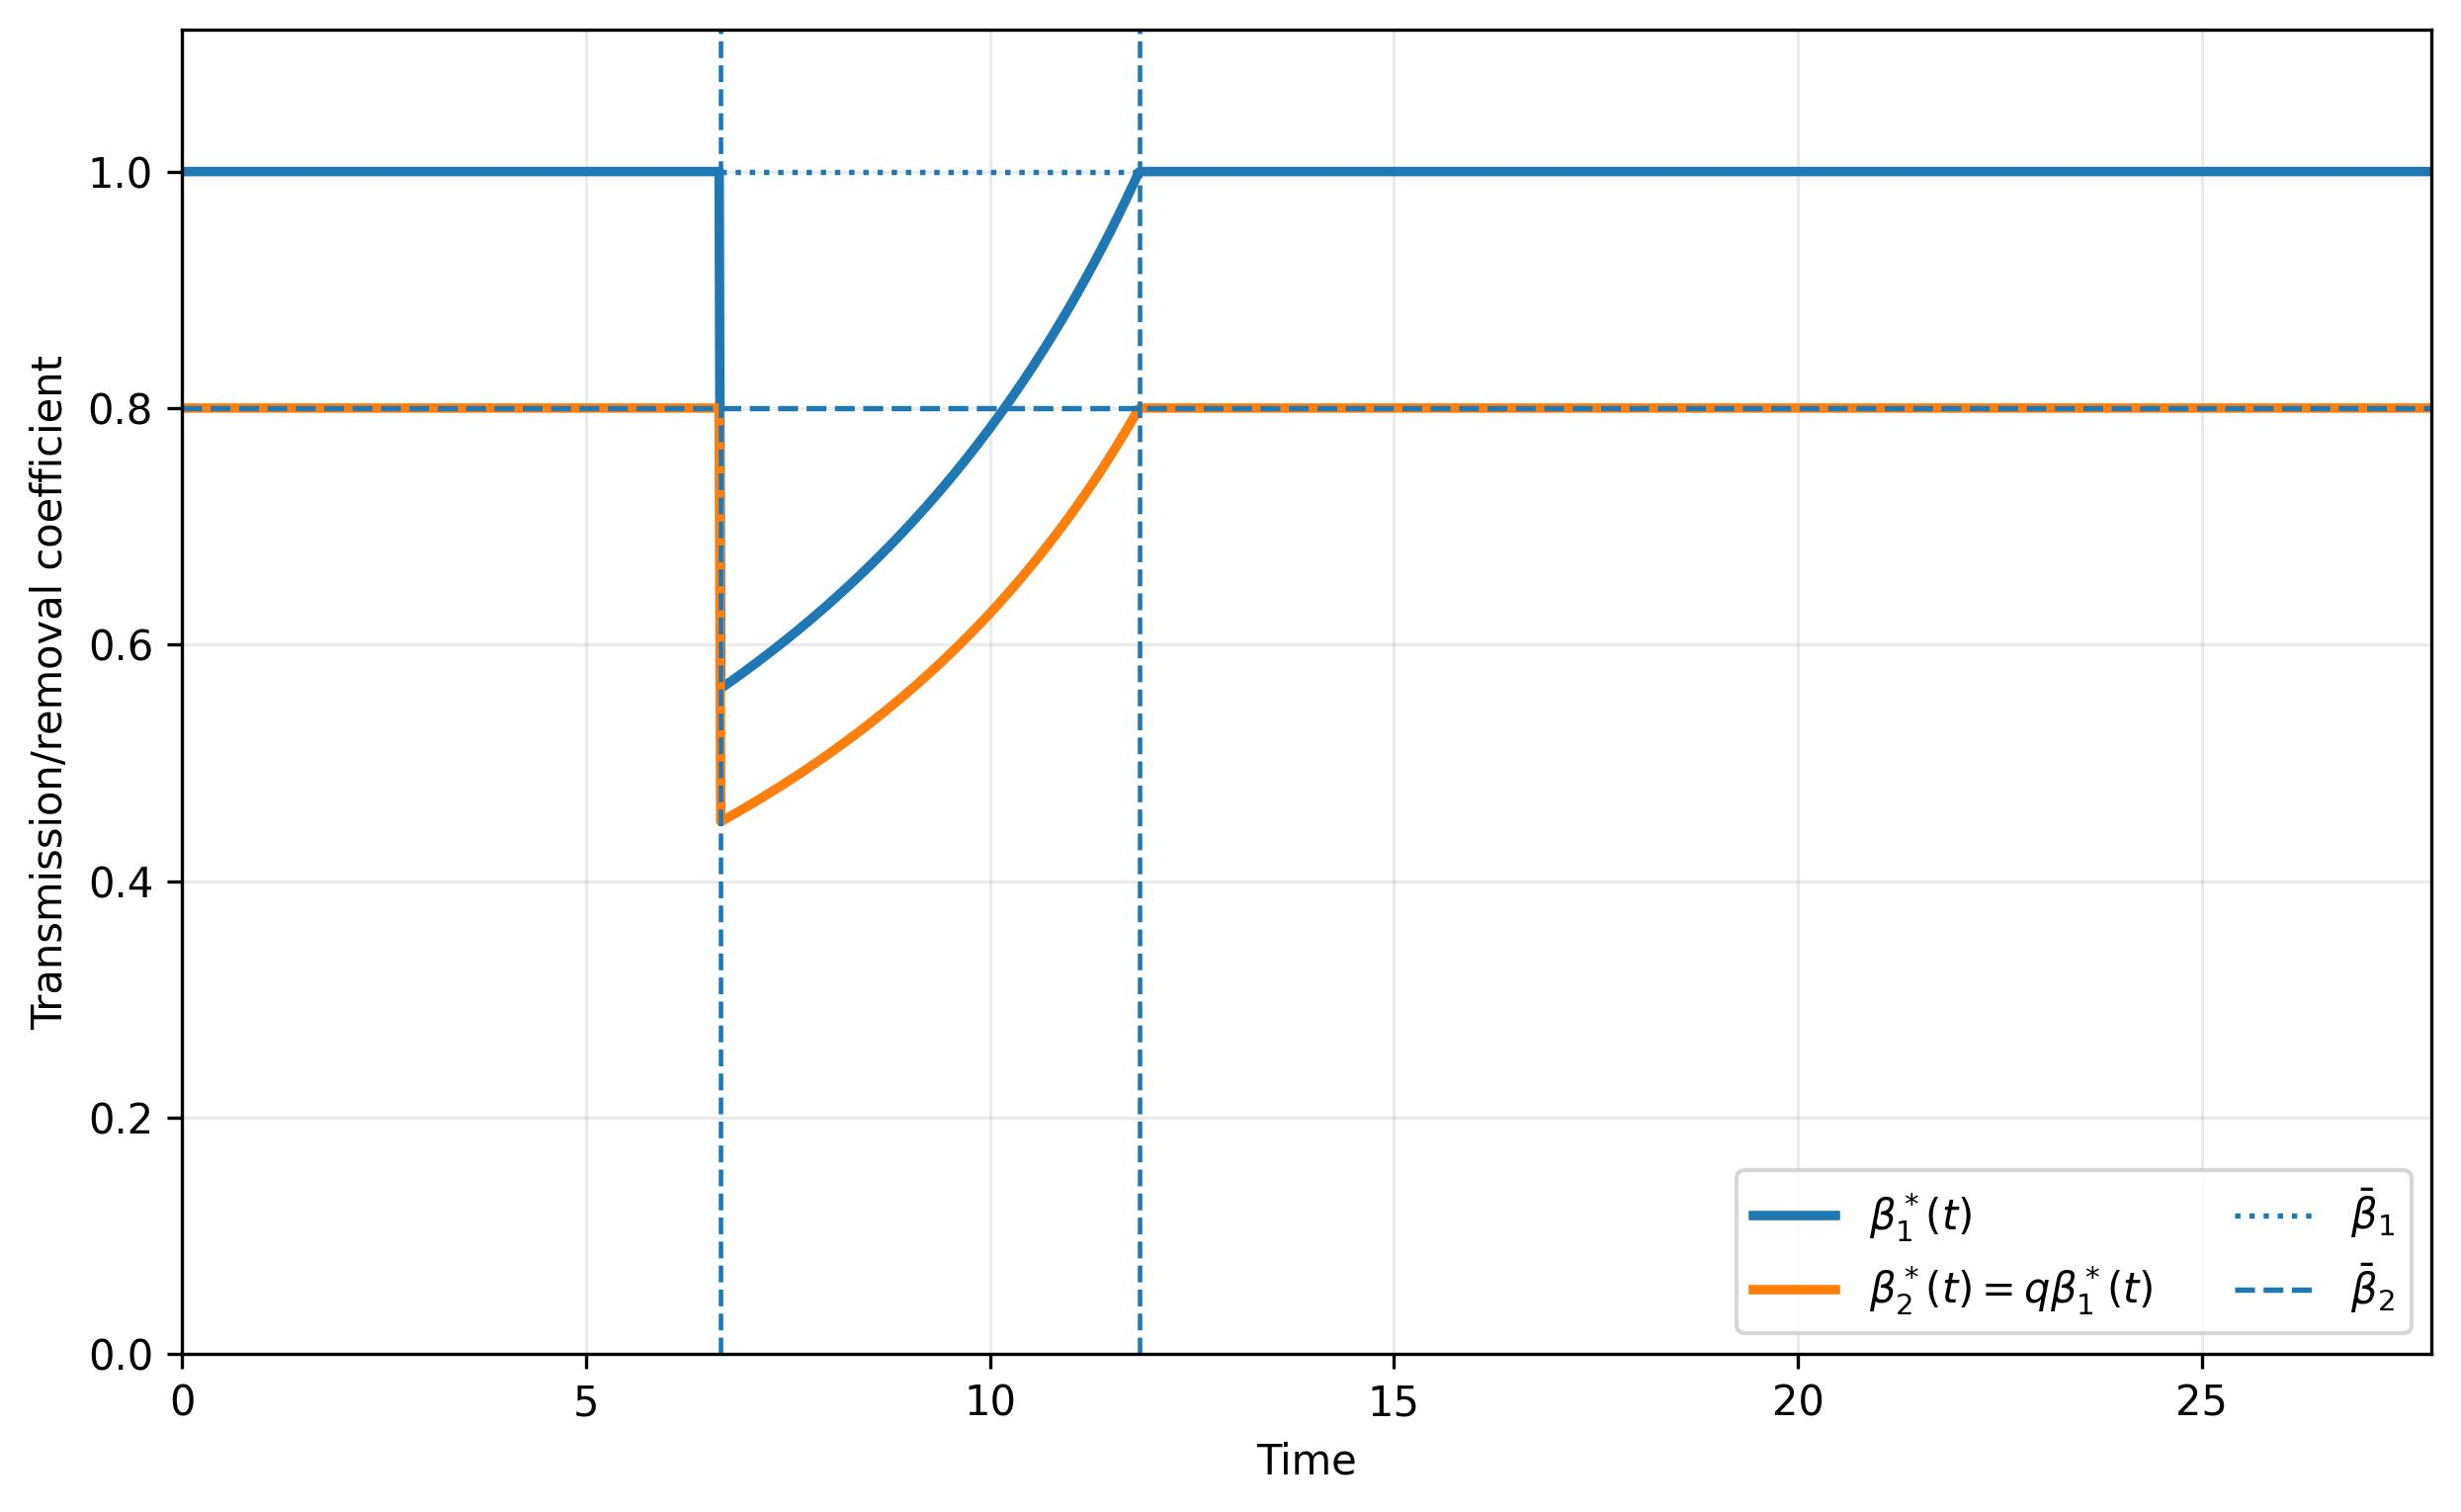
\includegraphics[width=0.92\textwidth]{Figure_3_optimal_controls.jpg}
\caption{两个不同的最优系数。$\beta_1^*$ 在 $\tau_1$ 发生向下跳跃，随后上升；$\beta_2^*=q\beta_1^*$ 保持固定比例，但数值始终不同。}
\label{fig:controls-time}
\end{figure}

\subsection{比较静态、唯一性与感染成本阈值}

\begin{figure}[H]
\centering
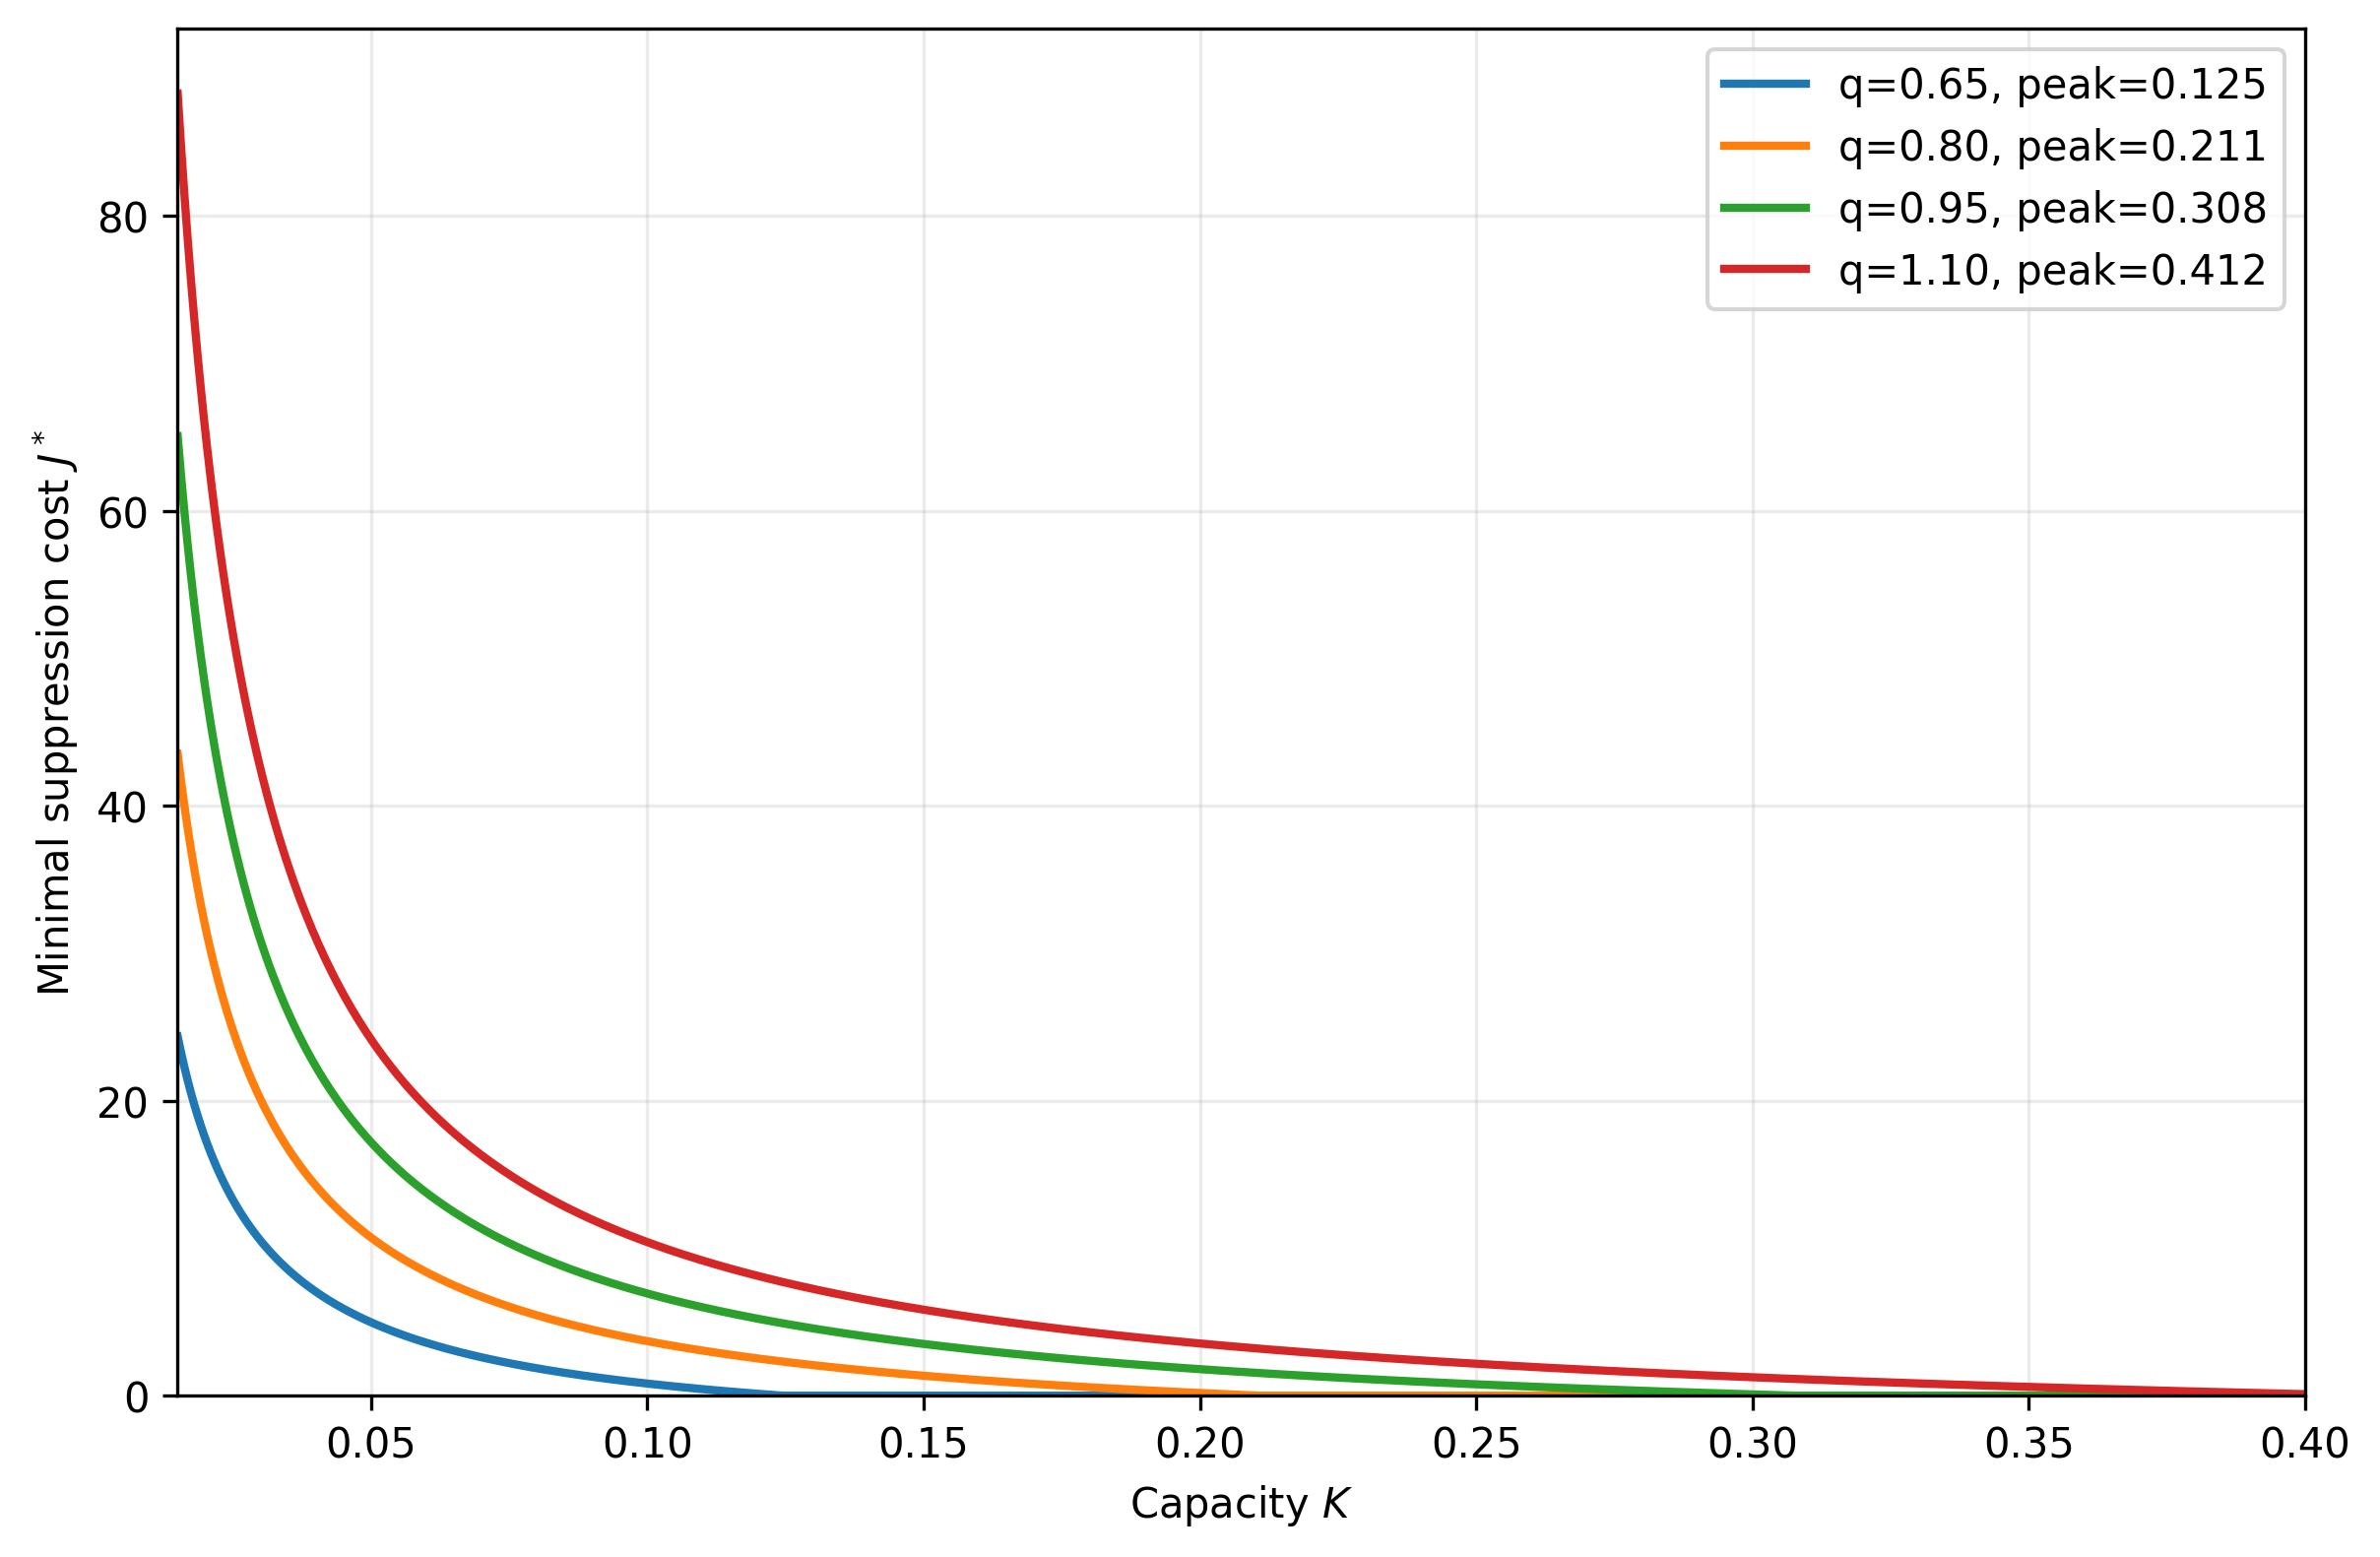
\includegraphics[width=0.92\textwidth]{Figure_4_cost_capacity.jpg}
\caption{不同 $q$ 下最小成本关于容量 $K$ 的变化。容量达到各自自然峰值后，最小成本降为零；$q$ 越大，峰值和控制成本越高。}
\label{fig:cost-capacity}
\end{figure}

为直观验证唯一性，考虑一族可行策略：自然传播首次达到某个 $h\le K$ 后，将感染维持在 $I=h$，直至 $x=x_h$。其成本为
\begin{equation}
C(h)=\frac1h\left[
\frac{B}{\gamma}(x_h^{\rm entry}-x_h)
-\ln\frac{x_h^{\rm entry}}{x_h}
\right],
\label{eq:plateau-family-cost}
\end{equation}
其中 $x_h^{\rm entry}$ 是自然轨道首次达到 $I=h$ 的横坐标。图~\ref{fig:plateau-cost} 显示 $C(h)$ 在允许区间内严格下降，因此唯一最小点是 $h=K$，即充分使用容量而不提前压低感染。

\begin{figure}[H]
\centering
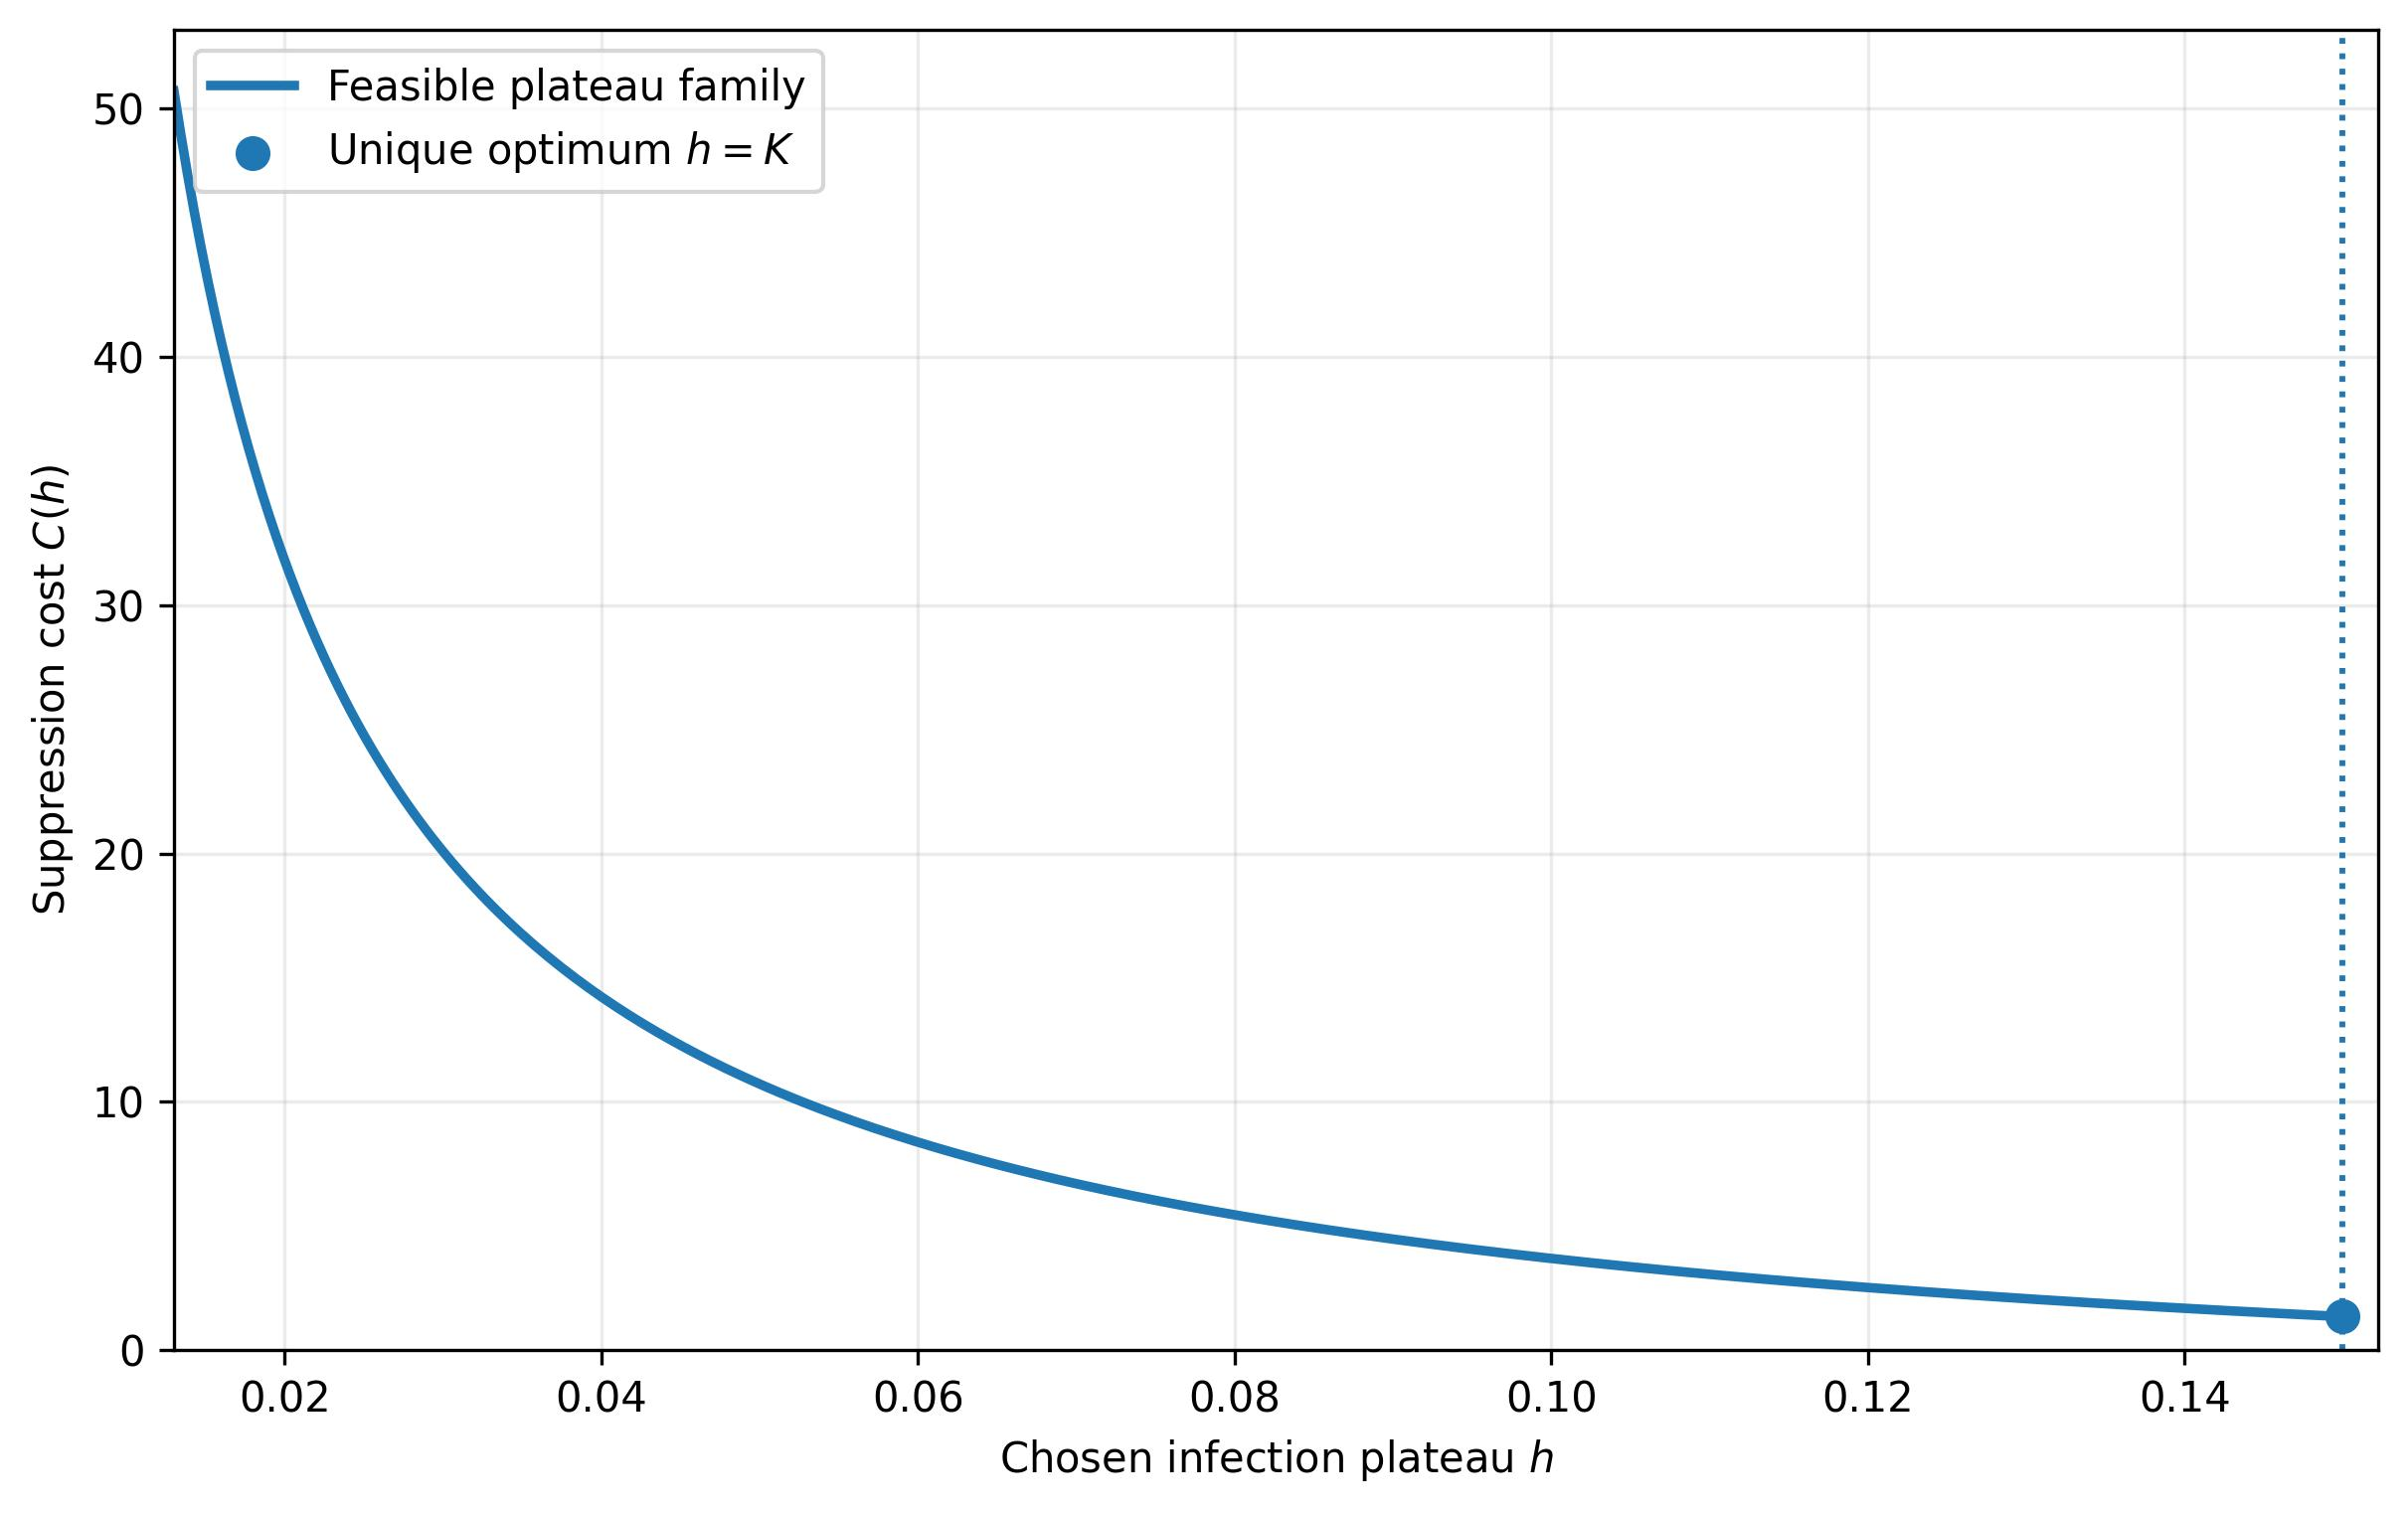
\includegraphics[width=0.92\textwidth]{Figure_5_uniqueness_plateau_cost.jpg}
\caption{可行平台策略的成本。唯一最小值发生在 $h=K$，与成本缺口恒等式\eqref{eq:gap-identity}一致。}
\label{fig:plateau-cost}
\end{figure}

\begin{figure}[H]
\centering
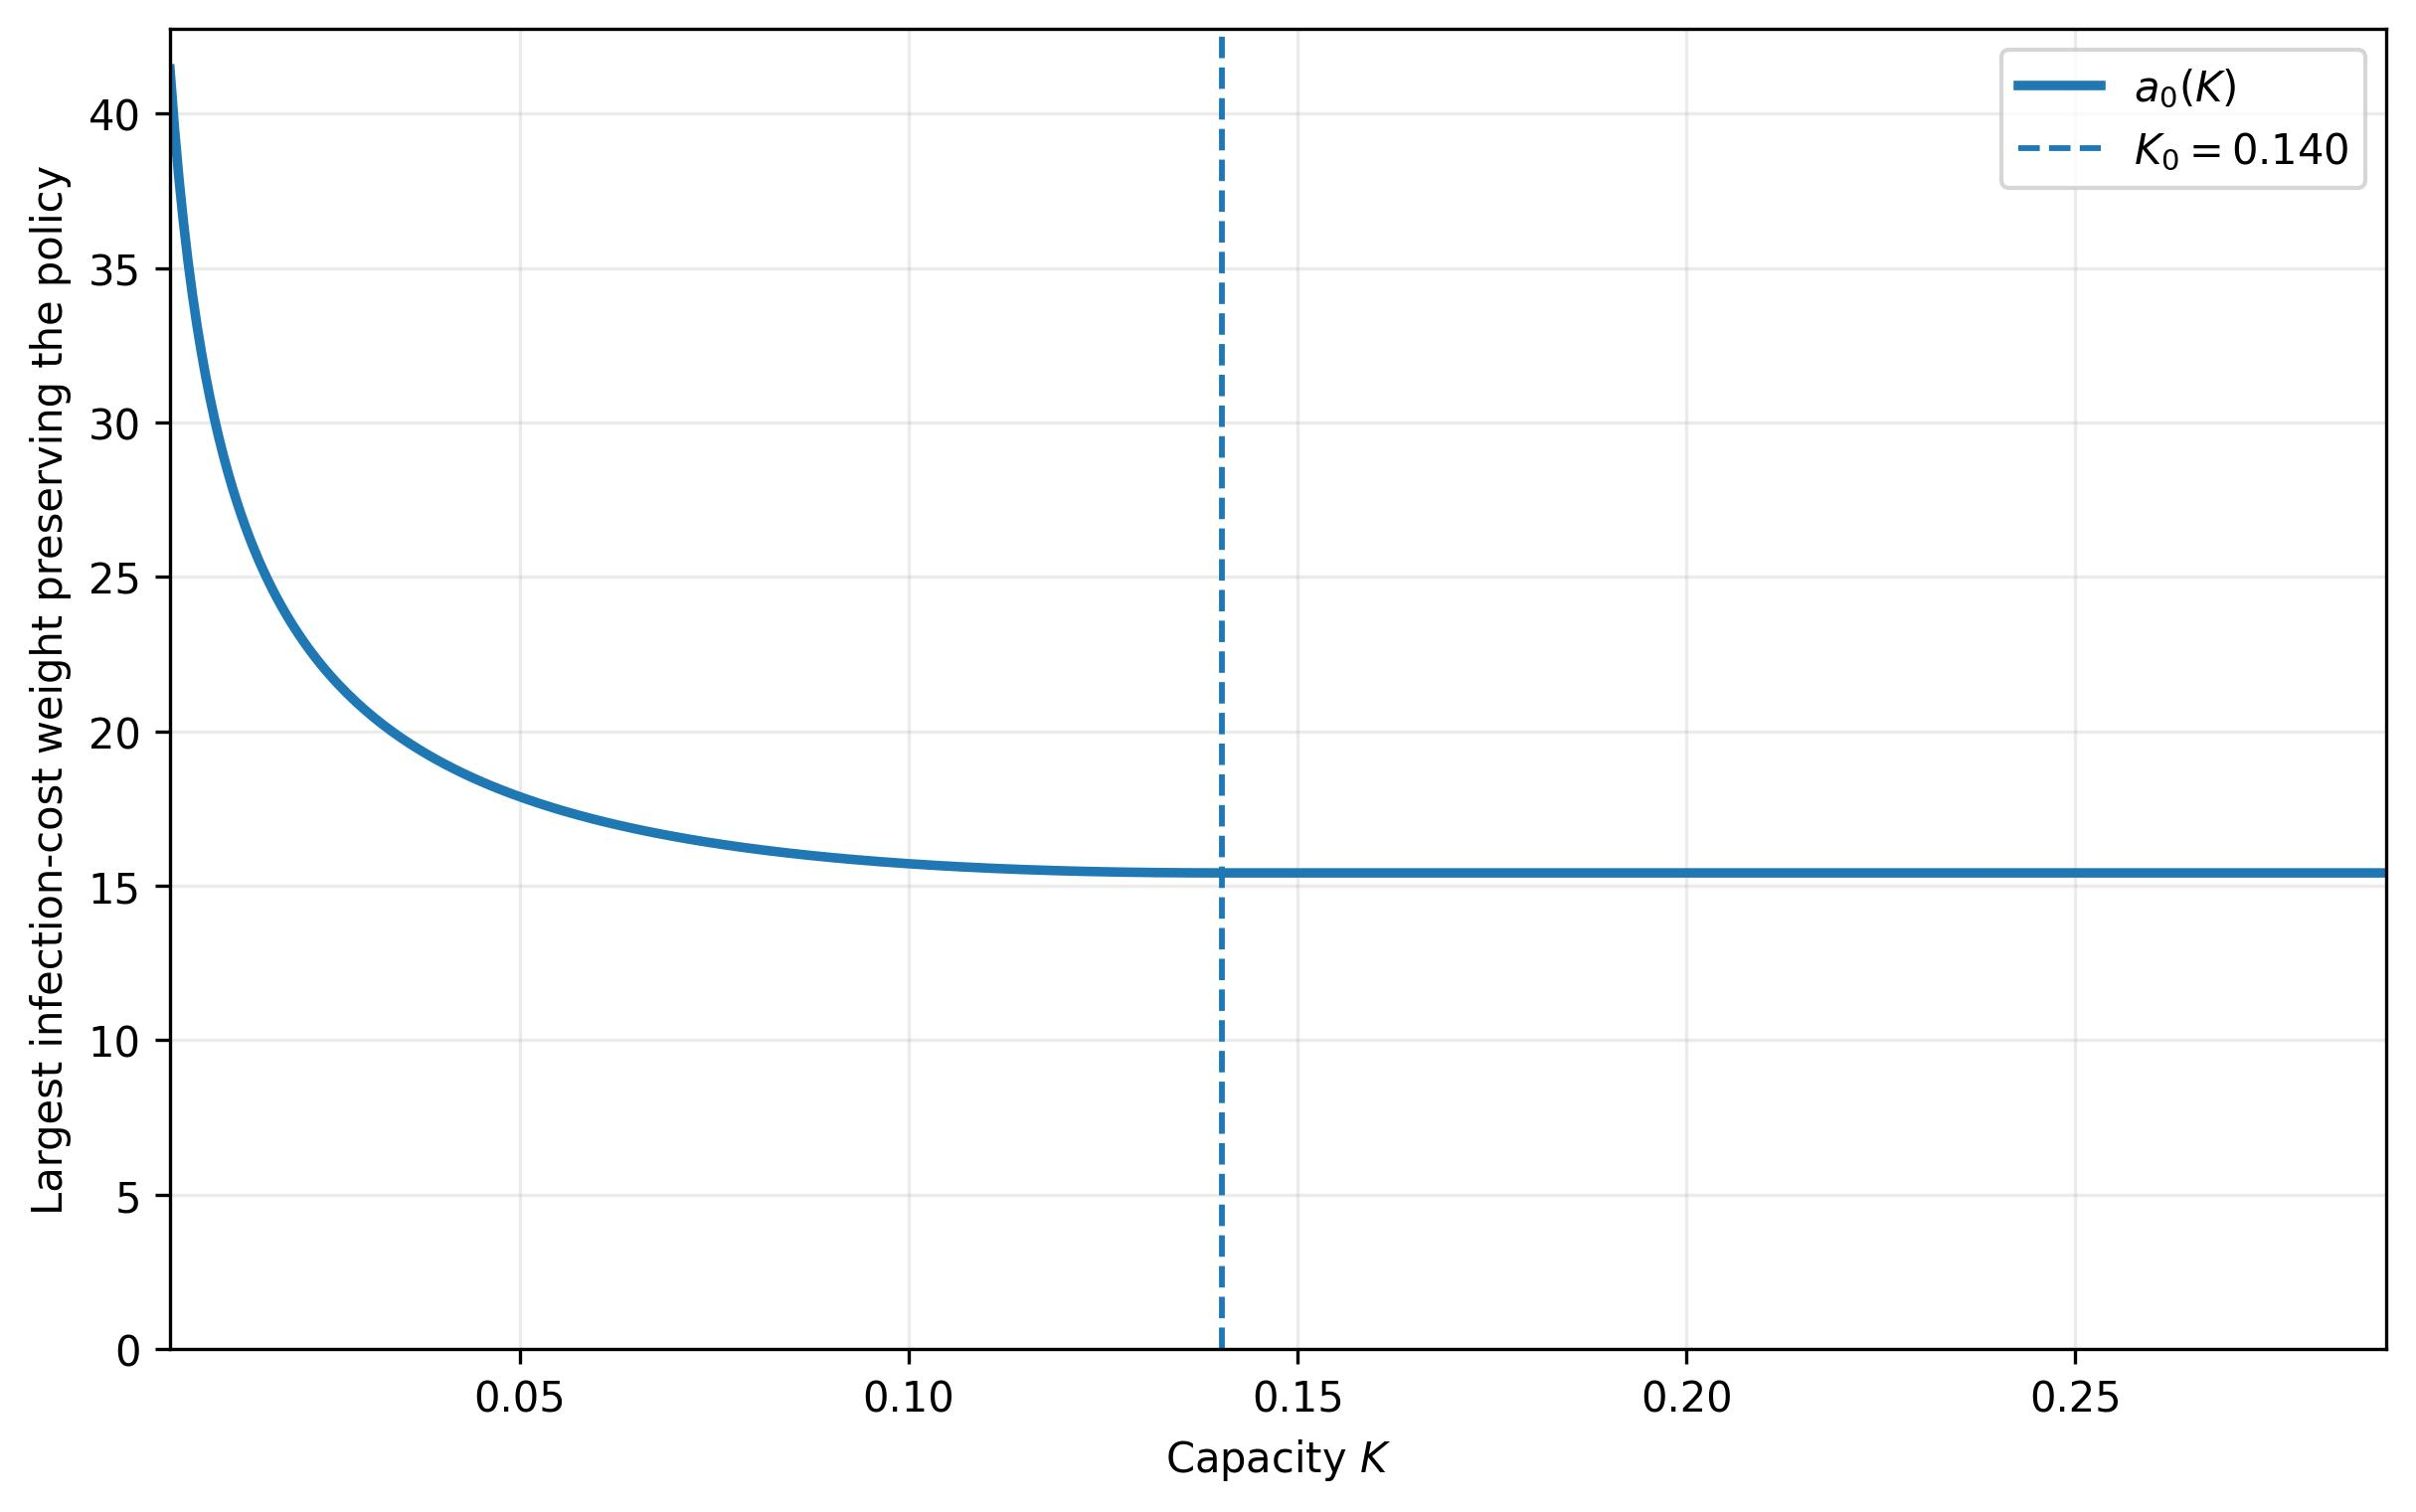
\includegraphics[width=0.92\textwidth]{Figure_6_infection_cost_threshold.jpg}
\caption{附加感染成本权重的稳健阈值 $a_0(K)$。在 $K\le K_0$ 区域阈值随容量上升而严格下降；超过 $K_0$ 后由一维极值的内部驻点决定并保持在平台值。}
\label{fig:a0}
\end{figure}

\subsection{独立控制的零成本反例}

图~\ref{fig:independent-nonunique} 取 $B_1=1$、$B_2=0.8$、$\gamma=0.3$、$(S_0,I_0)=(0.99,0.02)$、$K=0.15$。自然轨道显著突破容量。三个不同的短时 $\beta_1$ 加速脉冲都不降低任何系数，因此按\eqref{eq:independent-cost}成本均为零；它们却把 $S$ 快速降至 $\gamma/B_2$ 以下，使 $I$ 此后单调下降。该图不是数值优化现象，而是第~\ref{sec:independent-degeneracy}~节定理的直接构造。

\begin{figure}[H]
\centering
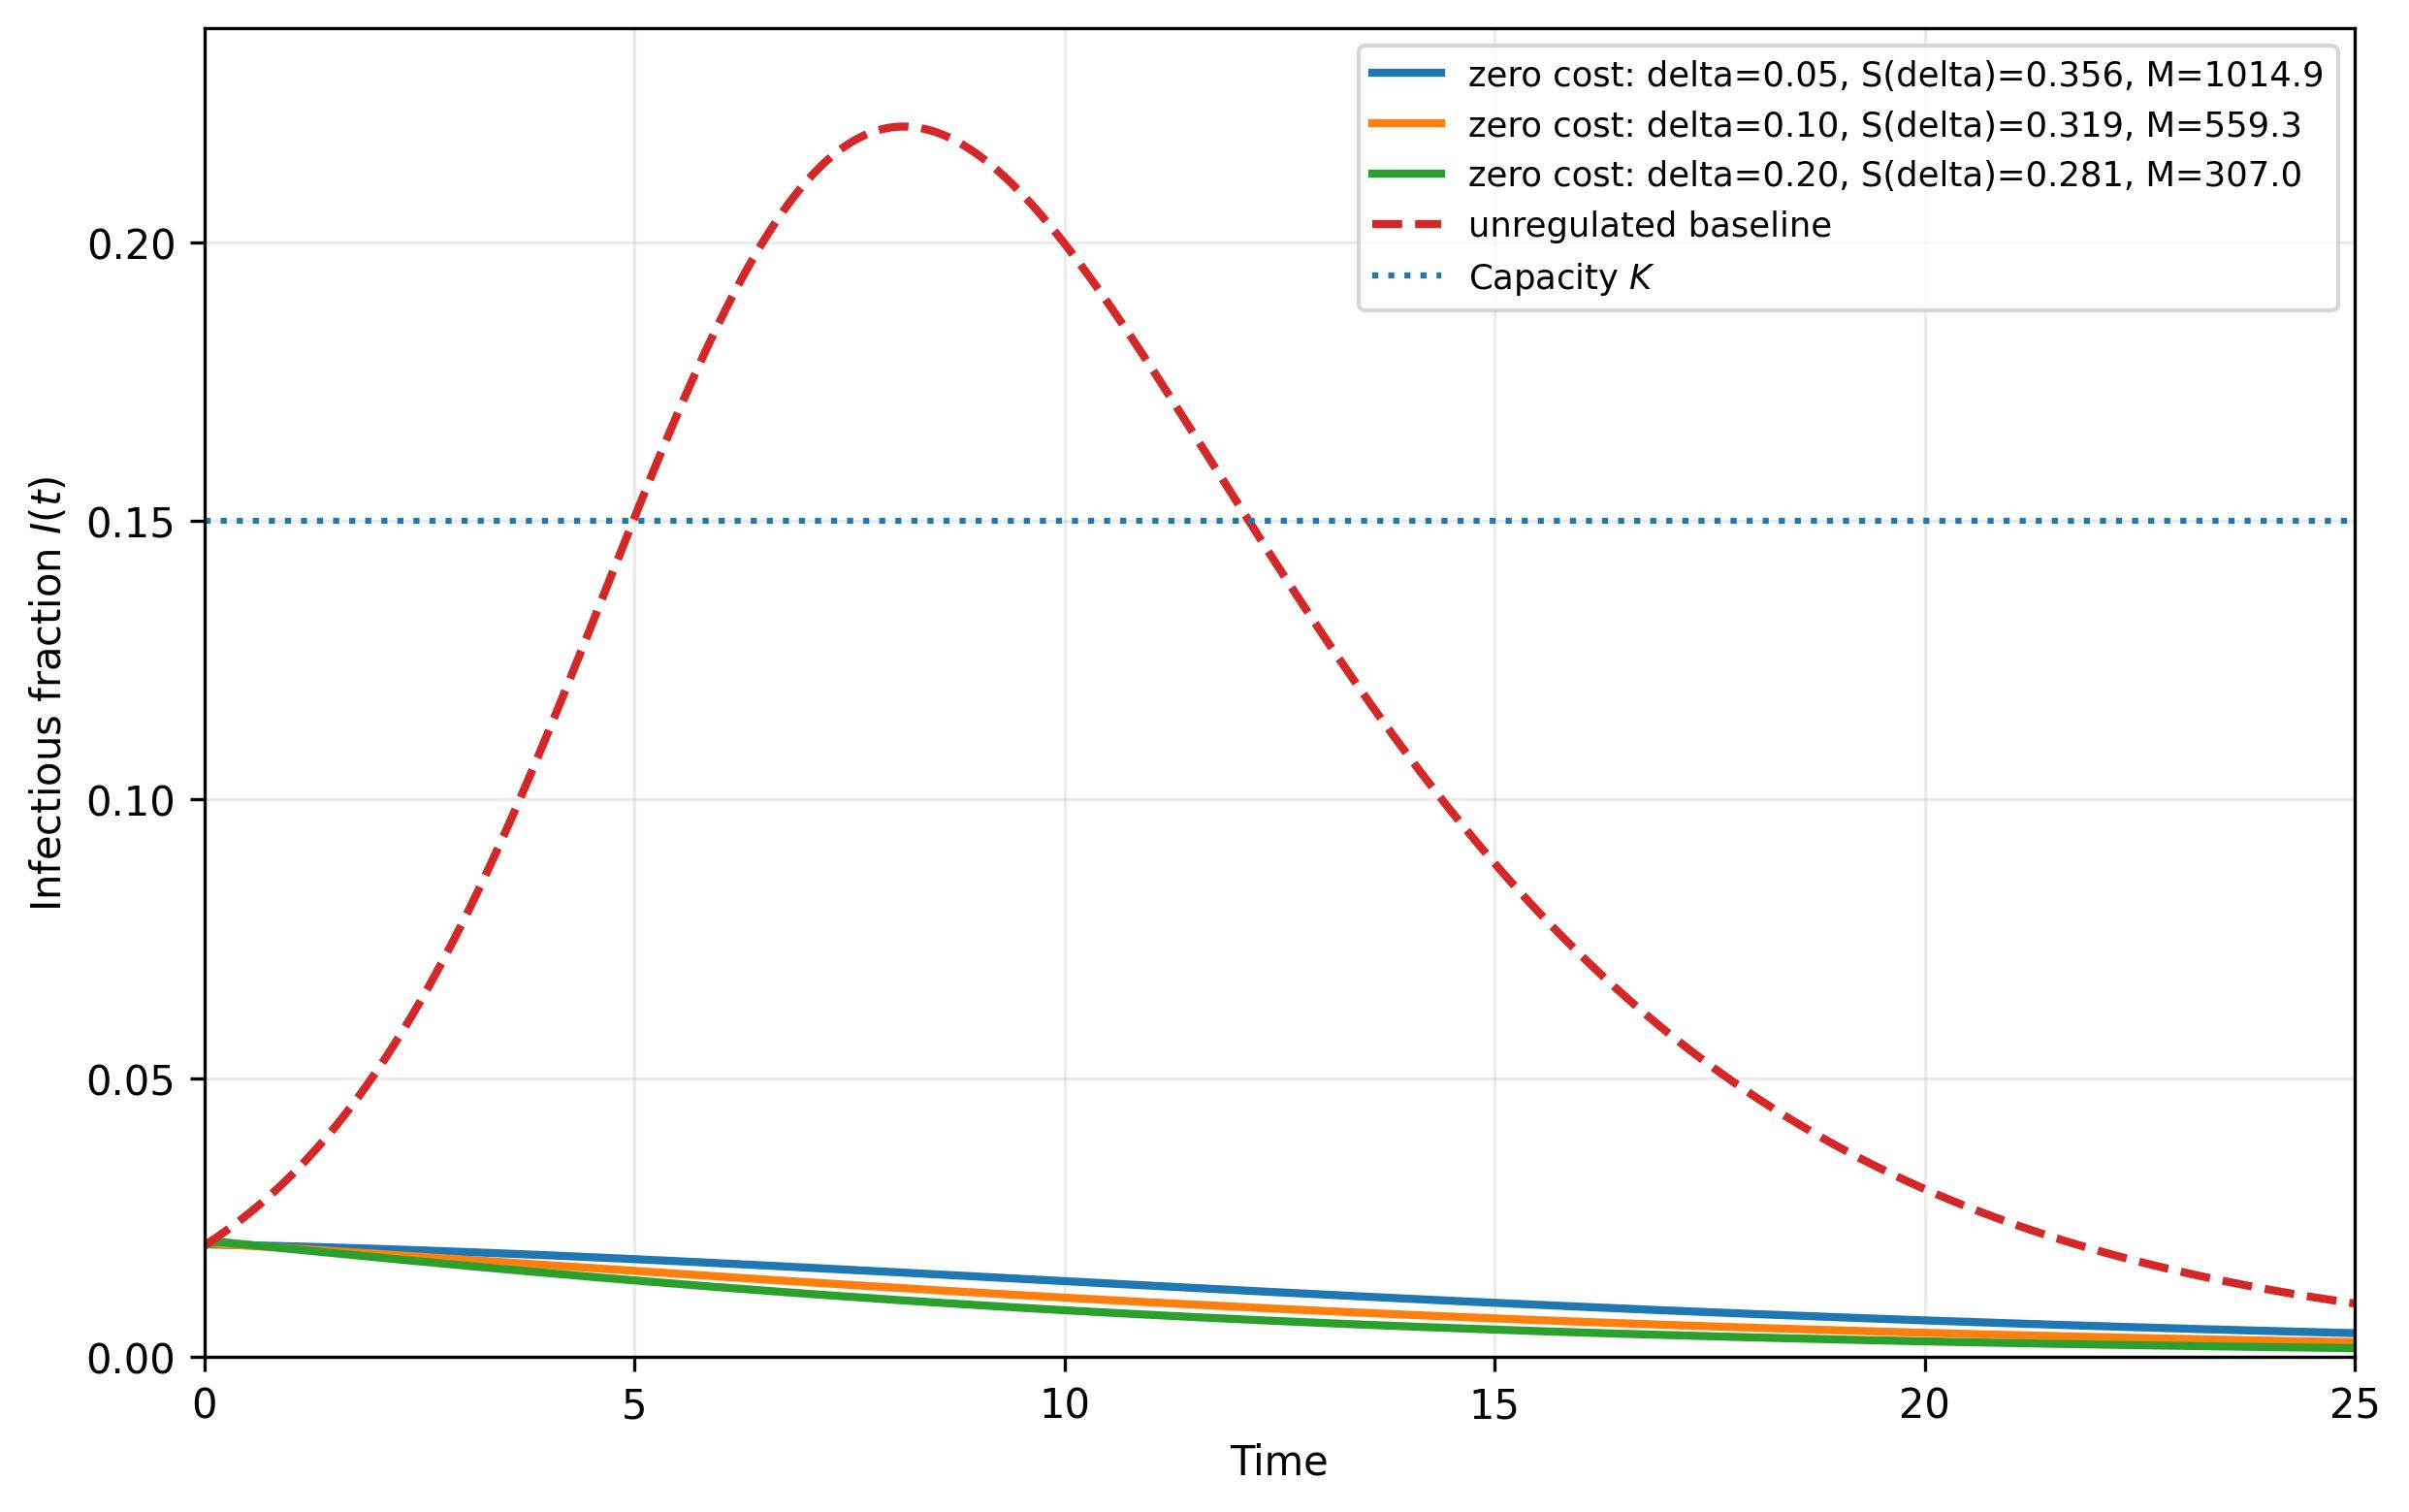
\includegraphics[width=0.92\textwidth]{Figure_7_independent_control_nonuniqueness.jpg}
\caption{完全独立控制下的零成本非唯一性。三条不同脉冲策略均满足容量且成本为零；虚线自然轨道则突破容量。}
\label{fig:independent-nonunique}
\end{figure}

\section{主要结论与建模建议}

\begin{enumerate}[label=\arabic*.,leftmargin=2.8em]
\item 对系统\eqref{eq:general-model}，\textbf{唯一性不是仅由微分方程决定的}，还取决于 $\beta_1$、$\beta_2$ 的耦合、允许范围和成本方向。
\item 在固定比例 $\beta_2=q\beta_1$ 下，令 $x=qS$ 后得到精确可解系统。最优策略仍是容量填充型，但两个最优系数在数值上不同：$\beta_2^*=q\beta_1^*$。
\item 新的校准不变量给出精确成本缺口\eqref{eq:gap-identity}。该恒等式同时证明全局最优性、首次两阶段唯一性，并量化提前抑制、过度抑制和无成本加速造成的损失。
\item 若限制 $0\le u\le B$，最优控制几乎处处全局唯一；若允许 $u>B$ 且加速不收费，解除控制之后仍有与附件论文同类的非唯一延拓。
\item 加入小的感染人数成本后，容量填充策略在 $a\le a_0(K)$ 范围内保持最优，阈值和最优值均有闭式表达；HJB 核查同时表明附件显示式中的阈值应取相应安全集上确界的倒数。
\item 若 $\beta_1$、$\beta_2$ 完全独立并继续使用正部线性成本，则存在无穷多个零成本最优控制，原有唯一性理论不能直接推广。此时必须加入上界、双向成本、固定耦合或缺失舱室。
\end{enumerate}

从应用角度，推荐先检验数据或机制是否支持近似固定比率
\(
\beta_2(t)/\beta_1(t)\approx q
\)。若支持，本文解析控制可直接用于参数敏感性和策略设计；若比率明显时变，应采用\eqref{eq:regularized-problem}一类有界正则化模型，并把“唯一性”表述为经过二阶充分条件验证的局部唯一性，而不应未经证明沿用同系数模型的全局唯一结论。

\appendix

\section{数值复现文件说明}

压缩包中的文件组织如下：
\begin{longtable}{p{0.31\textwidth}p{0.61\textwidth}}
\toprule
路径 & 内容\\
\midrule
\endfirsthead
\toprule
路径 & 内容\\
\midrule
\endhead
\nolinkurl{latex/main.tex} & 本文可编辑 LaTeX 主文件。\\
\nolinkurl{latex/references.bib} & 参考文献数据库。\\
\nolinkurl{figures/Figure_1--7.jpg} & 300 dpi 数值图。\\
\nolinkurl{python/Figure_1--7.py} & 每幅图独立运行的 Python 程序。\\
\nolinkurl{matlab/Figure_1--7.m} & 每幅图独立运行的 MATLAB 程序。\\
\nolinkurl{python/generate_numerical_summary.py} & 生成数值汇总表。\\
\nolinkurl{data/numerical_summary.csv} & 基准参数及关键输出。\\
\nolinkurl{README.md} & 编译与运行说明。\\
\bottomrule
\end{longtable}

\section{比例误差下的校准残差}

若实际关系为
\begin{equation}
\beta_2(t)=q\beta_1(t)+r(t),
\label{eq:ratio-mismatch}
\end{equation}
并仍以 $u=\beta_1$ 为政策变量，则 $x=qS$ 满足
\[
\dot x=-uxI,
\qquad
\dot I=uxI-\gamma I+r(t)S I.
\]
校准恒等式变为
\begin{equation}
\dot\Fcal=-x_hLI+x_hAI+r(t)SI.
\label{eq:mismatch-calibration}
\end{equation}
因此，固定比例模型不是对任意非比例系统的精确结论；但若 $r$ 在控制时段内较小，则其影响以显式残差积分进入。举例，若 $|r(t)|\le\varepsilon(t)$、$S\le S_0$、$I\le K$，则在首次到达 $x\le x_h$ 前
\begin{equation}
\left|\int r(t)S(t)I(t)\dd t\right|
\le S_0K\int\varepsilon(t)\dd t.
\label{eq:mismatch-bound}
\end{equation}
这给出了用数据检验固定比例近似时的误差尺度：应比较
\(
S_0K\|r\|_{L^1}
\)
与需要消除的校准差 $\Fcal_0-\Fcal_c$。

\section{一维计算的伪代码}

\begin{lstlisting}[basicstyle=\ttfamily\small,frame=single,breaklines=true]
Input: B, q, gamma, S0, I0, K
x0 = q*S0; xh = gamma/B
Ipeak = I0 + x0 - xh + xh*log(xh/x0)
if Ipeak <= K:
    u(t) = B; Jstar = 0
else:
    solve K = I0 + x0 - x1 + xh*log(x1/x0) for x1 > xh
    integrate laissez-faire until I=K to obtain tau1
    tau2 = tau1 + (x1-xh)/(gamma*K)
    u(t) = B                                  for t <= tau1
    u(t) = B/(1+B*K*(tau2-t))                 for tau1 < t <= tau2
    u(t) = B                                  for t > tau2
    beta1(t) = u(t); beta2(t) = q*u(t)
    Jstar = ((B/gamma)*(I0+x0-K)-log(B*x0/gamma)-1)/K
\end{lstlisting}

\bibliographystyle{plainnat}
\bibliography{references}

\end{document}
